% +--------------------------------------------------------------------+
% | LaTeX Template for K-State Electronic Theses, Dissertations,
% | and Reports
% |
% | Some guidelines for using the template are shown in comments.  Read
% | these comments carefully, as they describe changes you will need to
% | make to the template in order to meet Graduate School requirements.            |
% |
% | Additional information on using the template are contained in these
% | files, which are included when you download the template:
% |
% | ReadMe.pdf - A general overview of using the template
% |
% | BibTeX Guide.pdf - Detailed guidelines on using BibTeX to create
% | your bibliography and manage your citations.
% |
% | natbib.pdf - Gives detailed information on using the natbib package
% | and formatting citations
% +--------------------------------------------------------------------+

% +--------------------------------------------------------------------+
% | The template is designed to be used with PDFLaTeX. Process this
% | file (etdrtemplate.tex) with PDFLaTeX in order to produce a PDF
% | version of your ETDR.  If you are using BibTex to manage your
% | refrences, you will need to process your file four times:
% | 1. Run PDFLaTeX
% | 2. Run BibTex
% | 3. Run PDFLaTeX
% | 4. Run PDFLaTeX
% |
% | Some LaTeX editors do not explicitly list PDFLaTeX as an option, but
% | do use PDFLaTeX to produce a PDF file directly from your .tex files.
% | See the ReadMe file for details.
% +--------------------------------------------------------------------+
% |
% +--------------------------------------------------------------------+
% |
% | As required by the Graduate School, The template is configured to
% | contain the following sections in the order shown.

% | Abstract title page (doctoral dissertations only)
% | Abstract (doctoral dissertations only)
% | Title page
% | Copyright page
% | Abstract
% | Table of contents
% | List of figures
% | List of tables
% | Acknowledgements (Optional)
% | Dedication (Optional)
% | Preface (Optional)
% | Individual Chapters
% | References or Bibliography
% | Appendices (as needed)
% |
% | Details on removing optional sections are given in the comments below.
% |
% +--------------------------------------------------------------------+

% +--------------------------------------------------------------------+
% | The LaTex command \documentclass selects a particular class to
% | associate with the document.  Within this command, 12pt is
% | specified for the font size.  You can change this to 11 pt, if
% | desired.
% +--------------------------------------------------------------------+

\documentclass[final,letterpaper,12pt,oneside]{class_diss}

% +--------------------------------------------------------------------+
% | Here are added external packages that will be used throughout
% | the document.  You can add other packages as needed.
% +--------------------------------------------------------------------+

\usepackage{graphicx} % Extended graphics package.
\usepackage{amsmath} % American Mathematics Society standards
\usepackage{amsxtra} % Additional math symbols
\usepackage{amssymb} % Additional math symbols
\usepackage{amsthm} % Additional math symbols
\usepackage{latexsym} % Additional math symbols
\usepackage{setspace} % Controls line spacing
\usepackage[margin=1in]{geometry} % Sets page margins to 1 inch on all sides
\usepackage[titles]{tocloft} % Adds leader dots to all entries in the table of contents



%\usepackage{amsmath,amssymb,amscd,amsxtra,upref,stmaryrd}
%\usepackage{latexsym}
%\usepackage{mathtools}
%\usepackage[dvips]{graphics,epsfig}
%\usepackage{enumerate}
%\usepackage[colorlinks=true, pdfstartview=FitV, linkcolor=blue, citecolor=blue, urlcolor=blue]{hyperref}
%\usepackage{amsthm,amsfonts,color,esint,graphicx, float, mathabx}




% +--------------------------------------------------------------------+
% |
% | Citation and Bibliography Style
% |
% | The following commands determine the citation and bibliography style.  The
% | template uses BibTeX for formatting the bibliography.  See "BibTeX Guide.pdf"
% | for details on formatting citations and references.  The template is set
% | to use a generic, superscript style, but it can be easily modified
% | to use author-year styles.

\bibliographystyle{plain}
% | If you want to use an author-year citation style, change "unsrtnat" to
% | "plainnat" in the line above.  You can also use other styles supported
% | by LaTeX, e.g., acm, ieeetr, siam, etc.  Additional styles
% | are in the \styles folder and can be invoked like this:
% | \bibliographystyle{styles/apsrev}.  If the style you use is based
% | on an author-year citation style, you will need to make changes
% | in the usepackage and \setcitestyle statements below

\usepackage[super,sort&compress]{natbib}
% | If you want to use an author-year citation style, change "super" to
% | "authoryear" in the line above.

\setcitestyle{super}
% | if you want to use an author-year citation style, change "super" to
% | "authoryear" in the line above.

% +---------------------------------------------------------------------+
% | The hyperref package enables cross-references.
% +---------------------------------------------------------------------+

\usepackage[pdftex, plainpages=false, pdfpagelabels]{hyperref}

\hypersetup{
    linktocpage=true,
    colorlinks=true,
    bookmarks=true,
    citecolor=blue,
    urlcolor=blue,
    linkcolor=blue,
    citebordercolor={1 0 0},
    urlbordercolor={1 0 0},
    linkbordercolor={.7 .8 .8},
    breaklinks=true,
    pdfpagelabels=true,
    }


\newtheorem{theorem}{Theorem}[section]
\newtheorem{lemma}[theorem]{Lemma}
\newtheorem{proposition}[theorem]{Proposition}
\newtheorem{corollary}[theorem]{Corollary}


\newtheorem{thm}{Theorem} % used for known results
\renewcommand{\thethm}{\thesection.\Alph{thm}}
\newtheorem{lem}[thm]{Lemma} % used for known results
\newtheorem{prop}[thm]{Proposition} % used for known results
%\renewcommand{\thelem}{\Alph{lem}}


\theoremstyle{remark}
\newtheorem{dfn}{Definition}[section]
\newtheorem{example}{Example}[section]
\newtheorem{remark}{Remark}[section]
\renewcommand{\theequation}{\thesection.\arabic{equation}}

\newcommand{\comment}[1]{\vskip.3cm
\fbox{%
\parbox{0.93\linewidth}{\footnotesize #1}}
\vskip.3cm}

\newcommand{\blue}[1]{\textcolor{blue}{#1}}
\newcommand{\red}[1]{\textcolor{red}{#1}}



%Number sets, etc
\newcommand{\com}{\mathbb{C}}
\newcommand{\na}{\mathbb{N}}
\newcommand{\naz}{\mathbb{N}_0}
\newcommand{\re}{\mathbb{R}}
\newcommand{\ent}{\mathbb{Z}}
\newcommand{\toro}{\mathbb{T}}
\newcommand{\rn}{{{\mathbb R}^n}}
\newcommand{\rtn}{\re^{2n}}

%Function spaces
\newcommand{\sw}{{\mathcal{S}}(\rn)}
\newcommand{\swp}{{\mathcal{S}'}(\rn)}
\newcommand{\swz}{{\mathcal{S}_0}(\rn)}


%TL SPACES
\newcommand{\tlw}[4]{\dot F_{#1,#3}^{#2}(#4)} %weighted homogeneous Triebel-Lizorkin space: #1=p (L^p norm), #2=s (regularity), #3=q (l^q norm), #4=weight
\newcommand{\tl}[3]{\dot F_{#1,#3}^{#2}} %unweighted homogeneous Triebel-Lizorkin space
\newcommand{\itlw}[4]{F_{#1,#3}^{#2}(#4)} %weighted inhomogeneous Triebel-Lizorkin space: #1=p (L^p norm), #2=s (regularity), #3=q (l^q norm), #4=weight
\newcommand{\itl}[3]{F_{#1,#3}^{#2}} %unweighted inhomogeneous Triebel-Lizorkin space
%BESOV SPACES
\newcommand{\besw}[4]{\dot B_{#1,#3}^{#2}(#4)} %weighted homogeneous Besov space: #1=p (L^p norm), #2=s (regularity), #3=q (l^q norm), #4=weight
\newcommand{\bes}[3]{\dot B_{#1,#3}^{#2}} %unweighted homogeneous Besov space
\newcommand{\ibesw}[4]{B_{#1,#3}^{#2}(#4)} %weighted inhomogeneous Besov space: #1=p (L^p norm), #2=s (regularity), #3=q (l^q norm), #4=weight
\newcommand{\ibes}[3]{B_{#1,#3}^{#2}} %unweighted inhomogeneous Besov space

%LEBESGUE SPACES
\newcommand{\lebw}[2]{L^{#1}(#2)} %weighted Lebesgue space with #1=index and #2=weight 

%VARIABLE LEBESGUE SPACES
\newcommand{\Lp}{L^{p(\cdot)}} %variable Lp
\newcommand{\Lpc}{L^{p'(\cdot)}}
\newcommand{\Lq}{L^{q(\cdot)}} %variable Lq
\newcommand{\pp}{{p(\cdot)}}
\newcommand{\cpp}{{p'(\cdot)}}
\newcommand{\qq}{{q(\cdot)}}
\newcommand{\cqq}{{q'(\cdot)}}
\newcommand{\rr}{{r(\cdot)}}
\newcommand{\crr}{{r'(\cdot)}}
\newcommand{\ppo}{{p_1(\cdot)}}
\newcommand{\ppt}{{p_2(\cdot)}}

%MORREY SPACES
\newcommand{\mow}[3]{M_{#1}^{#2}(#3)}

%Cal letters
\newcommand{\C}{\mathcal{C}}
\newcommand{\M}{\mathcal{M}} % for the Hardy-Littelwood maximal function
\newcommand{\Mtau}{\mathcal{M}_\tau} 
\newcommand{\K}{\mathcal{K}}
\newcommand{\Ss}{\mathcal{S}}
%\newcommand{\P}{\mathcal{P}}
\newcommand{\B}{\mathcal{B}}
\def\P{\mathcal P}


%Greek letters
\newcommand{\f}{\varphi}
\newcommand{\fk}{\varphi_k}
\newcommand{\fj}{\varphi_j}


%Fourier transform of f and g; complex exponentials
\newcommand{\fhat}{\widehat{f}}
\newcommand{\ghat}{\widehat{g}}
\newcommand{\eixxi}{e^{2\pi i x \cdot \xi}}
\newcommand{\eixeta}{e^{2\pi i x \cdot \eta}}
\newcommand{\eixzeta}{e^{2\pi i x \cdot \zeta}}
\newcommand{\eixxe}{e^{2\pi i x \cdot (\xi + \eta)}}

%dx, etc
\newcommand{\dx}{\, dx}
\newcommand{\dy}{\, dy}
\newcommand{\dz}{\, dz}
\newcommand{\dxi}{\, d\xi}
\newcommand{\deta}{\, d\eta}
\newcommand{\dzeta}{\, d\zeta}



% Standard multiplier operators
\newcommand{\Do}[2]{\Delta^{#1}_{#2}}
\newcommand{\So}[2]{S^{#1}_{#2}}


%Other
\newcommand{\abs}[1]{\left\vert #1 \right\vert}
\newcommand{\fr}[2]{{\textstyle \frac{#1}{#2}}}
\newcommand{\norm}[2]{\left\|#1\right\|_{#2}}
\newcommand{\supp}{{\rm{supp}}}
\newcommand{\hc}{\frac{1}{p}=\frac{1}{p_1}+\frac{1}{p_2}}
\newcommand{\hcline}{1/p=1/p_1+1/p_2}
\newcommand{\tp}{\max\{0,n(\frac{1}{p}-1)\}}
\newcommand{\A}{D}
\newcommand{\ex}{d}
\newcommand{\gamt}{\gamma_{p_1,p_2,p,q}^{w_1,w_2, tl}}
\newcommand{\gamb}{\gamma_{p_1,p_2,p,q}^{w_1,w_2,b}}

\DeclareMathOperator*{\essinf}{ess\,inf}
\DeclareMathOperator*{\esssup}{ess\,sup}


%
%\textwidth6in
%
%\setlength{\topmargin}{0in} \addtolength{\topmargin}{-\headheight}
%\addtolength{\topmargin}{-\headsep}
%
%\setlength{\oddsidemargin}{0in}
%
%\oddsidemargin  0.0in \evensidemargin 0.0in \parindent0em
%
%\pagestyle{fancy}\lhead{Research Statement} \rhead{October 2018}
%\chead{{\large{\bf Alex Thomson}}} \lfoot{} \rfoot{\bf \thepage} \cfoot{}

\newcounter{list}

\setlength{\parindent}{2em}
\setlength{\parskip}{0em}
% +--------------------------------------------------------------------+
% | The document begins here.
% +--------------------------------------------------------------------+

\doublespacing
\begin{document}

% +--------------------------------------------------------------------+
% | ******Masters Students -- You Need to Make Some Changes Here******
% |
% | The Abstract Title page and Abstract page following the Abstract
% | Title page are required only for doctoral dissertations.  For
% | masters theses or reports, comment out or delete the lines:
% |
% | % +--------------------------------------------------------------------+
% | Abstract Title Page
% |
% |This page is required only for doctoral dissertations.
% +--------------------------------------------------------------------+

% +--------------------------------------------------------------------+
% | This page should not contain a page number.  We use the
% | \thispagestyle[empty] command below to suppress page numbers
% | and other style elements.
% +--------------------------------------------------------------------+

\thispagestyle{empty}

% +--------------------------------------------------------------------+
% | The Abstract Title page begins here
% +--------------------------------------------------------------------+

\pdfbookmark[0]{Title Page}{PDFTitlePage}
%\setcounter{page}{1}

\begin{center}

   \vspace{1cm}

% +--------------------------------------------------------------------+
% | Enter the title of your ETDR below.  For 2017 and on, use "Sentence case" (not ALL CAPS).
% | For details, see:  k-state.edu/grad/etdr/create/sentencecase.html 
% +--------------------------------------------------------------------+

   \large Bilinear pseudodifferential operators and Leibniz-type rules\\

   \vspace{0.5cm}

   by\\

   \vspace{0.5cm}

% +--------------------------------------------------------------------+
% | Enter your name below in standard name format (not ALL CAPS).
% +--------------------------------------------------------------------+

   \large Alexander Thomson\\

   \vspace{0.5cm}

% +--------------------------------------------------------------------+
% | On the line below, replace "Enter Your Previous Degrees"
% | with your previous degrees in mixed case. Include the abbreviation
% | for the degree, the name of the university, and the year separated
% | by commas. For example:
% |
% |    B.A., University of Illinois, 2000
% |
% | If desired, it is acceptable to include a city or country with
% | the university name. For example:
% |
% |    B.S., Jillian University, China, 2002
% |
% | Each degree should appear on a separate line.  Use the \\
% | command to create a line break.
% +--------------------------------------------------------------------+

  B.S., Missouri State University, 2013 \\
  M.S., Kansas State University, 2015\\

   \vspace{0.55cm}
   \rule{2in}{0.5pt}\\
   \vspace{0.75cm}

   {\large AN ABSTRACT OF A DISSERTATION}\\

   \vspace{0.5cm}
   \begin{singlespace}
   submitted in partial fulfillment of the\\
   requirements for the degree\\
   \end{singlespace}

   \vspace{0.5cm}

% +--------------------------------------------------------------------+
% | On the line below, enter the name of your earned degree in ALL
% | CAPITAL LETTERS.  For example: DOCTOR OF PHILOSOPHY
% +--------------------------------------------------------------------+


   {\large DOCTOR OF PHILOSOPHY}\\
   \vspace{0.5cm}

% +--------------------------------------------------------------------+
% | On the two lines below, enter the name of your department and the
% | name of the college in mixed case.  For example:
% |
% |     Biochemistry Department
% |     College of Arts and Sciences
% +--------------------------------------------------------------------+

   \begin{singlespace}
   		Department of Mathematics\\
   College of Arts and Sciences\\
   \end{singlespace}

   \vspace{0.5cm}

   \begin{singlespace}
   {\Large KANSAS STATE UNIVERSITY}\\
   Manhattan, Kansas\\
   \end{singlespace}

% +--------------------------------------------------------------------+
% | On the line below, replace "Graduation Year" with the four-digit year
% | of your graduation. For example:
% |
% |     2017
% +--------------------------------------------------------------------+

   2019\\
   \vspace{1cm}

\end{center}
 through \end{abstract}.
% |
% | You will also need to uncomment the two lines following the
% | \begin{abstract} command:
% |    %\setcounter{page}{-1}
% |    %\pdfbookmark[0]{Abstract}{PDFAbstractPage}
% |
% | Don't uncomment the lines above.  Scroll down several lines until
% | you see the section "For masters theses or reports, uncomment
% | the commands..." and uncomment the lines in that section.
% +--------------------- ----------------------------------------------+

% +--------------------------------------------------------------------+
% | Abstract Title Page
% |
% |This page is required only for doctoral dissertations.
% +--------------------------------------------------------------------+

% +--------------------------------------------------------------------+
% | This page should not contain a page number.  We use the
% | \thispagestyle[empty] command below to suppress page numbers
% | and other style elements.
% +--------------------------------------------------------------------+

\thispagestyle{empty}

% +--------------------------------------------------------------------+
% | The Abstract Title page begins here
% +--------------------------------------------------------------------+

\pdfbookmark[0]{Title Page}{PDFTitlePage}
%\setcounter{page}{1}

\begin{center}

   \vspace{1cm}

% +--------------------------------------------------------------------+
% | Enter the title of your ETDR below.  For 2017 and on, use "Sentence case" (not ALL CAPS).
% | For details, see:  k-state.edu/grad/etdr/create/sentencecase.html 
% +--------------------------------------------------------------------+

   \large Bilinear pseudodifferential operators and Leibniz-type rules\\

   \vspace{0.5cm}

   by\\

   \vspace{0.5cm}

% +--------------------------------------------------------------------+
% | Enter your name below in standard name format (not ALL CAPS).
% +--------------------------------------------------------------------+

   \large Alexander Thomson\\

   \vspace{0.5cm}

% +--------------------------------------------------------------------+
% | On the line below, replace "Enter Your Previous Degrees"
% | with your previous degrees in mixed case. Include the abbreviation
% | for the degree, the name of the university, and the year separated
% | by commas. For example:
% |
% |    B.A., University of Illinois, 2000
% |
% | If desired, it is acceptable to include a city or country with
% | the university name. For example:
% |
% |    B.S., Jillian University, China, 2002
% |
% | Each degree should appear on a separate line.  Use the \\
% | command to create a line break.
% +--------------------------------------------------------------------+

  B.S., Missouri State University, 2013 \\
  M.S., Kansas State University, 2015\\

   \vspace{0.55cm}
   \rule{2in}{0.5pt}\\
   \vspace{0.75cm}

   {\large AN ABSTRACT OF A DISSERTATION}\\

   \vspace{0.5cm}
   \begin{singlespace}
   submitted in partial fulfillment of the\\
   requirements for the degree\\
   \end{singlespace}

   \vspace{0.5cm}

% +--------------------------------------------------------------------+
% | On the line below, enter the name of your earned degree in ALL
% | CAPITAL LETTERS.  For example: DOCTOR OF PHILOSOPHY
% +--------------------------------------------------------------------+


   {\large DOCTOR OF PHILOSOPHY}\\
   \vspace{0.5cm}

% +--------------------------------------------------------------------+
% | On the two lines below, enter the name of your department and the
% | name of the college in mixed case.  For example:
% |
% |     Biochemistry Department
% |     College of Arts and Sciences
% +--------------------------------------------------------------------+

   \begin{singlespace}
   		Department of Mathematics\\
   College of Arts and Sciences\\
   \end{singlespace}

   \vspace{0.5cm}

   \begin{singlespace}
   {\Large KANSAS STATE UNIVERSITY}\\
   Manhattan, Kansas\\
   \end{singlespace}

% +--------------------------------------------------------------------+
% | On the line below, replace "Graduation Year" with the four-digit year
% | of your graduation. For example:
% |
% |     2017
% +--------------------------------------------------------------------+

   2019\\
   \vspace{1cm}

\end{center}
  % Masters students - comment or delete this line

\begin{abstract} % Masters students - comment or delete this line
   \setcounter{page}{-1} % Masters students - comment or delete this line
   \pdfbookmark[0]{Abstract}{PDFAbstractPage} % Masters students - comment or delete this line
   % +--------------------------------------------------------------------+
% | Abstract Page
% +--------------------------------------------------------------------+

\pagestyle{empty}
%\vspace{1cm}
\setlength{\baselineskip}{0.8cm}

%\indent

% +--------------------------------------------------------------------+
% | Enter the text of your abstract below.  There is no limit on the
% | number of words in your abstract.
% +--------------------------------------------------------------------+

Fractional Leibniz rules have been extensively studied due to their connections to partial
differential equations that model many real-world situations such as shallow water waves
and fluid flow. Broadly speaking, fractional Leibniz rules provide estimates of the size and smoothness of a product of functions in terms of the size and smoothness of the functions involved. In this dissertation, we obtain new Leibniz-type rules associated to bilinear pseudodifferential operators in a variety of function spaces that quantify smoothness and size in appropriate ways. Bilinear pseudodifferential operators combine functions through a symbol and the Fourier transform. When the symbol is identically equal to one, such operators give the product of two functions, and therefore, fractional Leibniz rules are particular cases of the Leibniz-type rules discussed.

The main results of this dissertation concern Leibniz-type rules for operators associated to two classes of symbols: Coifman-Meyer multipliers and symbols in the bilinear H\"ormander classes. Leibniz-type rules for Coifman-Meyer multiplier operators are presented in the setting of Triebel-Lizorkin and Besov spaces based on various quasi-Banach spaces that include weighted Lebesgue, weighted Lorentz, weighted Morrey, and variable-exponent Lebesgue spaces. Such results extend and improve previously known fractional Leibniz rules. As applications, we obtain scattering properties of solutions to certain systems of partial differential equations involving fractional powers of the Laplacian. For operators with symbols in the bilinear H\"ormander classes, we obtain Leibniz-type rules in the context of Besov and local Hardy spaces. The tools used in the proofs of the main results include Nikol'ski\u\i$\text{ }$ representations of function spaces, pointwise inequalities for maximal functions, and appropriate spectral decompositions of the symbols of the operators. % Masters students - comment or delete this line
   \vfill % Masters students - comment or delete this line
\end{abstract} % Masters students - comment or delete this line

% +--------------------------------------------------------------------+
% | Title Page -- Required for both Doctoral and Masters Students
% +--------------------------------------------------------------------+

% +--------------------------------------------------------------------+
% | Title Page
% +--------------------------------------------------------------------+

\newpage

% +--------------------------------------------------------------------+
% | This page should not contain a page number.  We use the
% | \thispagestyle[empty] command below to suppress page numbers
% | and other style elements.
% +--------------------------------------------------------------------+

\thispagestyle{empty}

% +--------------------------------------------------------------------+
% | The Title page begins here.
% +--------------------------------------------------------------------+

\begin{center}

   \vspace{1cm}

% +--------------------------------------------------------------------+
% | Enter the title of your ETDR below. For 2017 and on, use "Sentence case" (not ALL CAPS).
% | For details, see: k-state.edu/grad/etdr/create/sentencecase.html 
% +--------------------------------------------------------------------+

\large Leibniz-type rules in Triebel-Lizorkin and Besov spaces.\\

\vspace{0.5cm}

by\\

\vspace{0.5cm}

% +--------------------------------------------------------------------+
% | Enter your name below in standard name format (not ALL CAPS).
% +--------------------------------------------------------------------+

\large Alexander Thomson\\

 \vspace{0.3cm}

% +--------------------------------------------------------------------+
% | On the line below, replace "Enter Your Previous Degrees"
% | with your previous degrees in mixed case. Include the abbreviation
% | for the degree, the name of the university, and the year separated
% | by commas. For example:
% |
% |    B.A., University of Illinois, 2000
% |
% | If desired, it is acceptable to include a city or country with
% | the university name. For example:
% |
% |    B.S., Jillian University, China, 2002
% |
% | Each degree should appear on a separate line.  Use the \\
% | command to create a line break.
% +--------------------------------------------------------------------+

   B.S., Missouri State University, 2013\\
   M.S., Kansas State University, 2015\\

   \vspace{0.35cm}
   \rule{2in}{0.5pt}\\
   \vspace{0.65cm}

   {\large A DISSERTATION}\\

   \vspace{0.3cm}
   \begin{singlespace}
   submitted in partial fulfillment of the\\
   requirements for the degree\\
   \end{singlespace}

   \vspace{0.3cm}

% +--------------------------------------------------------------------+
% | On the line below, replace "ENTER YOUR DEGREE NAME" with the name
% | of your earned degree in ALL CAPITAL LETTERS.
% +--------------------------------------------------------------------+

   {\large DOCTOR OF PHILOSOPHY}\\
   \vspace{0.3cm}

% +--------------------------------------------------------------------+
% | On the two lines below, replace "Enter Your Department Name" and
% | "Enter Your College Name" with the name of your department and the
% | name of the college in mixed case.  For example:
% |
% |     Biochemistry Department
% |     College of Arts and Sciences
% +--------------------------------------------------------------------+

   \begin{singlespace}
   Department of Mathematics\\
   College of Arts and Sciences\\
   \end{singlespace}

   \vspace{0.3cm}

   \begin{singlespace}
   {\large KANSAS STATE UNIVERSITY}\\
   Manhattan, Kansas\\
   \end{singlespace}

% +--------------------------------------------------------------------+
% | On the line below, replace "Graduation Year" with the four-digit
% | year of your graduation.  For example:
% |
% |     2016
% +--------------------------------------------------------------------+

   2019\\
   \vspace{0.3cm}

    \end{center}

    \begin{flushright}
    Approved by:\\
    \vspace{0.3cm}
    \begin{singlespace}
    Major Professor


% +--------------------------------------------------------------------+
% | On the line below, replace "Enter Your Major Professor's Name"
% | with  the name of your major professor in mixed case.  Use the
% | format Firstname Lastname.  For example:
% |
% |     Lori Goetsch
% |
% +--------------------------------------------------------------------+

    Enter Your Major Professor's Name\\
    \end{singlespace}
    \end{flushright}

% +--------------------------------------------------------------------+
% | If you have co-major professors, comment out the lines above from
% | \begin{flushright} through \end{flushright} and uncomment the
% | lines below.  Enter your co-major professors' names where indicated.
% +--------------------------------------------------------------------+

%\begin{flushright}
%   Approved by:\\
%  \vspace{ 0.3cm}
%   \begin{singlespace}
%   Co-Major Professor\\
%   Enter Your Co-Major Professor's Name\\
%   \vspace{.25cm}
%   Co-Major Professor\\
%   Enter Your Co-Major Professor's Name\\
%   \end{singlespace}
%\end{flushright}


% +--------------------------------------------------------------------+
% | Copyright Page -- Required for both Doctoral and Masters Students
% +--------------------------------------------------------------------+

%\input{copyright.tex}

% +--------------------------------------------------------------------+
% |  Abstract -- Required for both Doctoral and Masters Students
% +--------------------------------------------------------------------+

\begin{abstract}

% +--------------------------------------------------------------------+
% | For masters theses or reports, uncomment the commands on the next
% | two lines (\setcounter and \pdfbookmark)
% +--------------------------------------------------------------------+

   %\setcounter{page}{-1}
   %\pdfbookmark[0]{Abstract}{PDFAbstractPage}

% +--------------------------------------------------------------------+
% | Abstract Page
% +--------------------------------------------------------------------+

\pagestyle{empty}
%\vspace{1cm}
\setlength{\baselineskip}{0.8cm}

%\indent

% +--------------------------------------------------------------------+
% | Enter the text of your abstract below.  There is no limit on the
% | number of words in your abstract.
% +--------------------------------------------------------------------+

Fractional Leibniz rules have been extensively studied due to their connections to partial
differential equations that model many real-world situations such as shallow water waves
and fluid flow. Broadly speaking, fractional Leibniz rules provide estimates of the size and smoothness of a product of functions in terms of the size and smoothness of the functions involved. In this dissertation, we obtain new Leibniz-type rules associated to bilinear pseudodifferential operators in a variety of function spaces that quantify smoothness and size in appropriate ways. Bilinear pseudodifferential operators combine functions through a symbol and the Fourier transform. When the symbol is identically equal to one, such operators give the product of two functions, and therefore, fractional Leibniz rules are particular cases of the Leibniz-type rules discussed.

The main results of this dissertation concern Leibniz-type rules for operators associated to two classes of symbols: Coifman-Meyer multipliers and symbols in the bilinear H\"ormander classes. Leibniz-type rules for Coifman-Meyer multiplier operators are presented in the setting of Triebel-Lizorkin and Besov spaces based on various quasi-Banach spaces that include weighted Lebesgue, weighted Lorentz, weighted Morrey, and variable-exponent Lebesgue spaces. Such results extend and improve previously known fractional Leibniz rules. As applications, we obtain scattering properties of solutions to certain systems of partial differential equations involving fractional powers of the Laplacian. For operators with symbols in the bilinear H\"ormander classes, we obtain Leibniz-type rules in the context of Besov and local Hardy spaces. The tools used in the proofs of the main results include Nikol'ski\u\i$\text{ }$ representations of function spaces, pointwise inequalities for maximal functions, and appropriate spectral decompositions of the symbols of the operators.
\vfill
\end{abstract}

% +--------------------------------------------------------------------+
% | The following commands start a new page and set the page numbering
% | to lowercase roman numerals.
% +--------------------------------------------------------------------+

\newpage
\pagenumbering{roman}

% +--------------------------------------------------------------------+
% |
% | *********************** IMPORTANT ******************************
% |
% | In the \setcounter command below, set the number to represent the
% | page number of the table of contents page.  For example, if the
% | table of contents page is the 6th page of your document, enter 6
% | in the brackets.  This number may vary, depending on the length of
% | your abstract.
% |
% | Numbers do not appear on the title and abstract pages, but they
% | are included in the page count.  The table of contents page is the
% | first page on which page numbers are displayed.
% +--------------------------------------------------------------------+

\setcounter{page}{6}

% +--------------------------------------------------------------------+
% | The following command creates a bookmark for the table of contents
% | in the final PDF document.
% +--------------------------------------------------------------------+

\pdfbookmark[0]{\contentsname}{contents}

% +--------------------------------------------------------=-----------+
% | The following command adds dot leaders for all entries in the
% | table of contents.
% +--------------------------------------------------------------------+

\renewcommand{\cftchapleader}{\cftdotfill{\cftdotsep}}

% +--------------------------------------------------------------------+
% | The following commands makes all entries and page numbers in the
% | table of contents appear in normal weight font (not bold).
% +--------------------------------------------------------------------+

\renewcommand{\cftchapfont}{\mdseries}
\renewcommand{\cftchappagefont}{\mdseries}

% +--------------------------------------------------------------------+
% | These commands add the table of contents, list of figures, and
% | list of tables.
% +--------------------------------------------------------------------+

\tableofcontents
\listoffigures
\listoftables

% +--------------------------------------------------------------------+
% | Acknowledgements Page
% |
% | If you choose not to have an Acknowledgements page, comment out
% | or delete the following 3 lines.
% +--------------------------------------------------------------------+

%\newpage
%\phantomsection
%\addcontentsline{toc}{chapter}{Acknowledgements}
%% +--------------------------------------------------------------------+
% | Acknowledgements Page (Optional)
% +--------------------------------------------------------------------+

\newpage
\vspace*{0.9cm}
\begin{center}
{\bf \Huge Acknowledgments}
\end{center}

\setlength{\baselineskip}{0.8cm}

%\pdfbookmark[0]{Acknowledgements}{PDF_Acknowledgements}

% +--------------------------------------------------------------------+
% | Enter text for your acknowledgements in the space below this box.
% |                                                                    
% +--------------------------------------------------------------------+

Enter the text for your Acknowledgements page in the acknowledge.tex
file. The Acknowledgements page is optional.  If you wish to remove
it, see the comments in the etdrtemplate.tex file.


% +--------------------------------------------------------------------+
% | Dedication Page
% |
% | If you choose not to have a Dedication page, comment out
% | or delete the following 3 lines.
% +--------------------------------------------------------------------+

%\newpage
%\phantomsection
%\addcontentsline{toc}{chapter}{Dedication}
%% +--------------------------------------------------------------------+
% | Dedication Page (Optional)
% +--------------------------------------------------------------------+

\newpage
\vspace*{0.9cm}
\begin{center}
{\bf \Huge Dedication}
\end{center}

\setlength{\baselineskip}{0.8cm}

%\pdfbookmark[0]{Dedication}{PDF_Dedication}

% +--------------------------------------------------------------------+
% | Enter the text for your dedication in the space below this box.    
% +--------------------------------------------------------------------+

Enter the text for your Dedication page in the dedication.tex file.
The Dedication page is optional.  If you wish to remove it, see the
comments in the etdrtemplate.tex file.


% +--------------------------------------------------------------------+
% | Preface Page
% |
% | If you choose not to have a Dedication page, comment out
% | or delete the following 4 lines.
% +--------------------------------------------------------------------+

%\newpage
%\phantomsection
%\addcontentsline{toc}{chapter}{Preface}
%% +--------------------------------------------------------------------+
% | Preface (Optional)
% +--------------------------------------------------------------------+

\newpage
\vspace*{0.9cm}
\begin{center}
{\bf \Huge Preface}
\end{center}

\setlength{\baselineskip}{0.8cm}

%\pdfbookmark[0]{Preface}{PDF_Preface}

% +--------------------------------------------------------------------+
% | Enter text of your Preface in the space below this box.            
% +--------------------------------------------------------------------+

Enter the text for your Preface page in the preface.tex file. The
Preface page is optional.  If you wish to remove it, see the
comments in the etdrtemplate.tex file.



% +--------------------------------------------------------------------+
% | This is where the chapter content of your ETDR begins.
% +--------------------------------------------------------------------+

%\phantomsection
\newpage
\pagenumbering{arabic}
\setcounter{page}{1}

% +--------------------------------------------------------------------+
% | Individual chapters of your ETDR are added using the \input
% | command.
% +--------------------------------------------------------------------+

% +--------------------------------------------------------------------+
% | Sample Chapter 1
% |
% | This file provides examples of how to
% | - insert a figure with a caption
% | - construct a table with a caption
% | - create subsections within the chapter
% | - insert a reference to a Figure or Table
% | - make a citation
% +--------------------------------------------------------------------+

\cleardoublepage

% +--------------------------------------------------------------------+
% | Replace "Chapter Title" below with the title of your chapter.
% | LaTeX will automatically number the chapters.
% +--------------------------------------------------------------------+

\chapter{Introduction to Leibniz-type rules}
\label{makereference1}

Leibniz-type rules have been extensively studied due to their connections to partial differential equations which model many real world situations such as shallow water waves and fluid flow. In this chapter we introduce some of the definitions and history of the development of Leibniz-type rules which motivated the results to be discussed in chapters 2 and 3 of this manuscript. First consider the Leibniz rule taught in Calculus courses which expresses the derivatives of a product of functions as a linear combination of derivatives of the functions involved; more specifically, for functions $f$ and $g$ sufficiently smooth, it holds that
\[\partial^\alpha_x (fg)(x) = \sum_{\alpha_1 + \alpha_2 = \alpha} C_{\alpha_1 \alpha_2} \partial^{\alpha_1}_x f(x) \partial^{\alpha_2}_x g(x),\]
where $\alpha \in \mathbb{N}^n_0$ and $C_{\alpha_1 \alpha_2}$ are appropriate constants. The definitions in of the function spaces used below and multiindices $\alpha\in\mathbb{N}^n_0$ will be discussed in Appendix A \ref{Appendix:Key1}. In particular one term has all the derivatives on $f$ and another with $\alpha$ derivatives on $g$ and
\[ \partial^\alpha_x (fg)(x) = \partial^\alpha_x f(x) g(x) + f(x) \partial^\alpha_x g(x) + ...\]
In an analogous way, fractional Leibniz rules give estimates of the smoothness and size of a product of functions in terms of the smoothness and size of the factors. For instance, for $f$ and $g$ in the Schwartz class $\mathcal{S}(\mathbb{R}^n)$, it holds that
\begin{equation}\label{def:leibniz}
\norm{D^s (fg)}{L^r} \lesssim \norm{D^s f}{L^{p_1}}\norm{g}{L^{q_1}} + \norm{f}{L^{p_2}}\norm{D^s g}{L^{q_2}},
\end{equation}
where $1/r = 1/p_1 + 1/q_1 = 1/p_2 + 1/q_2$, $1<p_1,p_2,q_1,q_2\leq \infty$, $1/2 <r\leq \infty$, and $s>N(1/min(r,1) - 1)$ or $s$ is an even natural number. The homogeneous fractional differentiation operator of order $s$, $D^s$, is defined as \[D^s f(x) = \int_\rn |\xi|^s \widehat{f}(\xi) e^{2\pi i x\cdot \xi} d\xi,\]
where $\widehat{f}$ is the Fourier transform of $f$.
For $s>0$, the operator $D^s$ is naturally understood as taking $s$ derivatives of its argument. Indeed, in the case $s=2$, $D^2f = c\Delta f$, where $\Delta = \sum_{j=1}^n \partial^2_{x_j}$ is the Laplacian operator. Furthermore, if $s$ is a positive integer,

%the $\dot{W}^{k,p}$ norm and $\norm{D^k \cdot}{L^p}$ are equivalent norms where 
%\[\norm{f}{\cdot{W}^{k,p}} = \sum_{|\alpha|=k} \norm{\partial^\alpha}{L^p}.\] 

\[\norm{D^s f}{L^p} \sim \sum_{|\alpha| = s} \norm{\partial^\alpha f}{L^p},\]
where $|\alpha| = \alpha_1 + \alpha_2 + ... + \alpha_n$ for $\alpha = (\alpha_1,\alpha_2,...,\alpha_n) \in \mathbb{N}^n_0.$

 Another version of (\ref{def:leibniz}) is obtained by using the inhomogeneous sth order fractional differentiation operator $J^s$:
\begin{equation}\label{def:ileibniz}
\norm{J^s(fg)}{L^r} \lesssim \norm{J^s f}{L^{p_1}}\norm{g}{L^{q_1}} + \norm{f}{L^{p_2}}\norm{J^s g}{L^{q_2}}.
\end{equation}
Similarly to its homeogenous counterpart, the operator $J^s$ is defined through the Fourier transform as 
\[ J^s f(x) = \int_{\rn} (1+|\xi|^2)^\frac{s}{2} \widehat{f}(\xi)e^{2\pi i x\cdot\xi} d\xi\]
and can be interpreted as taking derivatives up to order $s$ of $f$.
%Then $s>0$ it is interpreted as taking up to $s$ derivatives of the function it is applied to as when $s=k$ is a positive integer $\norm{J^k(f)}{L^p} = \norm{f}{W^{k,p}}$ where $\norm{f}{W^{k,p}} = \sum_{|\alpha|\leq k} \norm{\partial^\alpha f}{L^p}$.
 
The estimates (\ref{def:leibniz}) and (\ref{def:ileibniz}) are also known as Kato-Ponce inequalities due to the foundational work of Kato-Ponce \cite{MR951744}, where the estimate (\ref{def:ileibniz}) was proved in the case $1<r=p_1=q_2<\infty$ and $p_2=q_1=\infty$, with applications to the Cauchy problem for Euler and Navier-Stokes equations. This result was extended by Gulisashvili-Kon \cite{MR1420922}, who showed (\ref{def:leibniz}) and (\ref{def:ileibniz}) for the cases $s>0$, $1<r<\infty$, and $1 < p_1,p_2,q_1,q_2\leq\infty$ in connection to smoothing properties of Schr\"odinger semigroups. Grafakos-Oh \cite{MR3200091} and Muscalu-Schlag \cite{MR3052499} established the cases for $1/2 <r\leq 1$ and the case $r=\infty$ was completed in the work of Bourgain-Li \cite{MR3263081} and Grafakos-Maldonado-Naibo \cite{MR3189525}. Applications of the estimates (\ref{def:leibniz}) and (\ref{def:ileibniz}) to Korteweg-de Vries equations were studied by Christ-Weinstein \cite{MR1124294} and Kenig-Ponce-Vega \cite{MR1211741}.

In the estimates (\ref{def:leibniz}) and (\ref{def:ileibniz}) the two functions $f$ and $g$ are related through pointwise multiplication. Throughout the rest of this manuscript we will consider estimates similar to (\ref{def:leibniz}) and (\ref{def:ileibniz}) where the two functions are related through a pseudodifferntial operator. Let $\sigma(x,\xi,\eta)$ be a complex-valued, smooth function for $x,\xi,\eta\in\rn$. We define the \textit{bilinear pseudodifferential operator}  associated to $\sigma$, $T_\sigma$, by 
\[T_{\sigma}(f,g)(x) = \int_{\mathbb{R}^{2n}} \sigma(x,\xi,\eta) \widehat{f}(\xi)\widehat{g}(\eta)e^{-2\pi i x\cdot(\xi+\eta)}d\xi d\eta. \]
We refer to $\sigma$ as the symbol of the operator $T_\sigma$. When $\sigma$ is independent of $x$ we call $\sigma$ the multiplier of the \textit{bilinear multiplier operator} $T_\sigma$. 


Throughout this manuscript we will study estimates related to (\ref{def:leibniz}) and (\ref{def:ileibniz}) associated to bilinear pseudodifferential operators that are of the form 
\begin{equation}\label{h_general_estimate}
\norm{D^s T_\sigma(f,g)}{Z} \lesssim \norm{D^sf}{X_1}\norm{g}{Y_1} + \norm{f}{X_2}\norm{D^s g}{Y_2} ,
\end{equation}
\begin{equation}\label{i_general_estimate}
\norm{J^sT_\sigma(f,g)}{Z} \lesssim \norm{J^sf}{X_1}\norm{g}{Y_1} + \norm{f}{X_2}\norm{J^sg}{Y_2} ,
\end{equation}
for a variety of function spaces $X_1$, $X_2$, $Y_1$, $Y_2$, and $Z$.

%When $\sigma \equiv 1$, the Fourier inversion formula implies that $T_\sigma(f,g) = fg$. Therefore, estimates of the form (\ref{h_general_estimate}) and (\ref{i_general_estimate}) include, as particular cases, the estimates (\ref{def:leibniz}) and (\ref{def:ileibniz}) presented in Section 1 by choosing $Z$, $X_1$, $Y_1$, $X_2$, and $Y_2$ to be appropriate Lebesgue spaces.

The estimates (\ref{h_general_estimate}) and (\ref{i_general_estimate}) have been extensively studied in a variety of settings. In \cite{MR3750234}, Brummer-Naibo studied Leibniz-type rules in function spaces that admit a molecular decomposition and a $\varphi$-transform characterization in the sense of Frazier-Jawerth \cite{MR808825, MR1070037}. In the context of Lebesgue spaces and mixed Lebesgue spaces, estimates of the type (\ref{h_general_estimate}) were studied in Hart-Torres-Wu \cite{HTW} for bilinear multiplier operators with minimal smoothness assumptions on the multipliers. Related mapping properties for bilinear pseudodifferential operators with symbols in the bilinear H\"ormander classes were studied by B\'enyi-Torres \cite{MR1986065} and B\'enyi-Nahmod-Torres \cite{MR2250054} in the setting of Sobolev spaces, by B\'enyi \cite{MR1996120} in the setting of Besov spaces, and by Naibo \cite{MR3393696} and Koezuka-Tomita \cite{MR3750316} in the context of Triebel-Lizorkin spaces. Additionally, versions of (\ref{def:leibniz}) and (\ref{def:ileibniz}) in weighted Lebesgue spaces were proved in Cruz-Uribe-Naibo \cite{MR3513582}, while Brummer-Naibo \cite{BrNa2017} proved (\ref{h_general_estimate}) and (\ref{i_general_estimate}) in weighted Lebesgue spaces for Coifman-Meyer multiplier operators. 

In chapter two we will present Leibniz-type rules in the settings of Besov and Triebel-Lizorkin spaces based in various function spaces. The techniques used are quite flexible and allow the method of proof to be adapted to many different function spaces. 

In chapter three we will present Leibniz-type rules in Besov spaces for bilinear pseudodifferential operators symbols of critical order.

%\begin{figure}[htb]%t=top, b=bottom, h=here
%
%    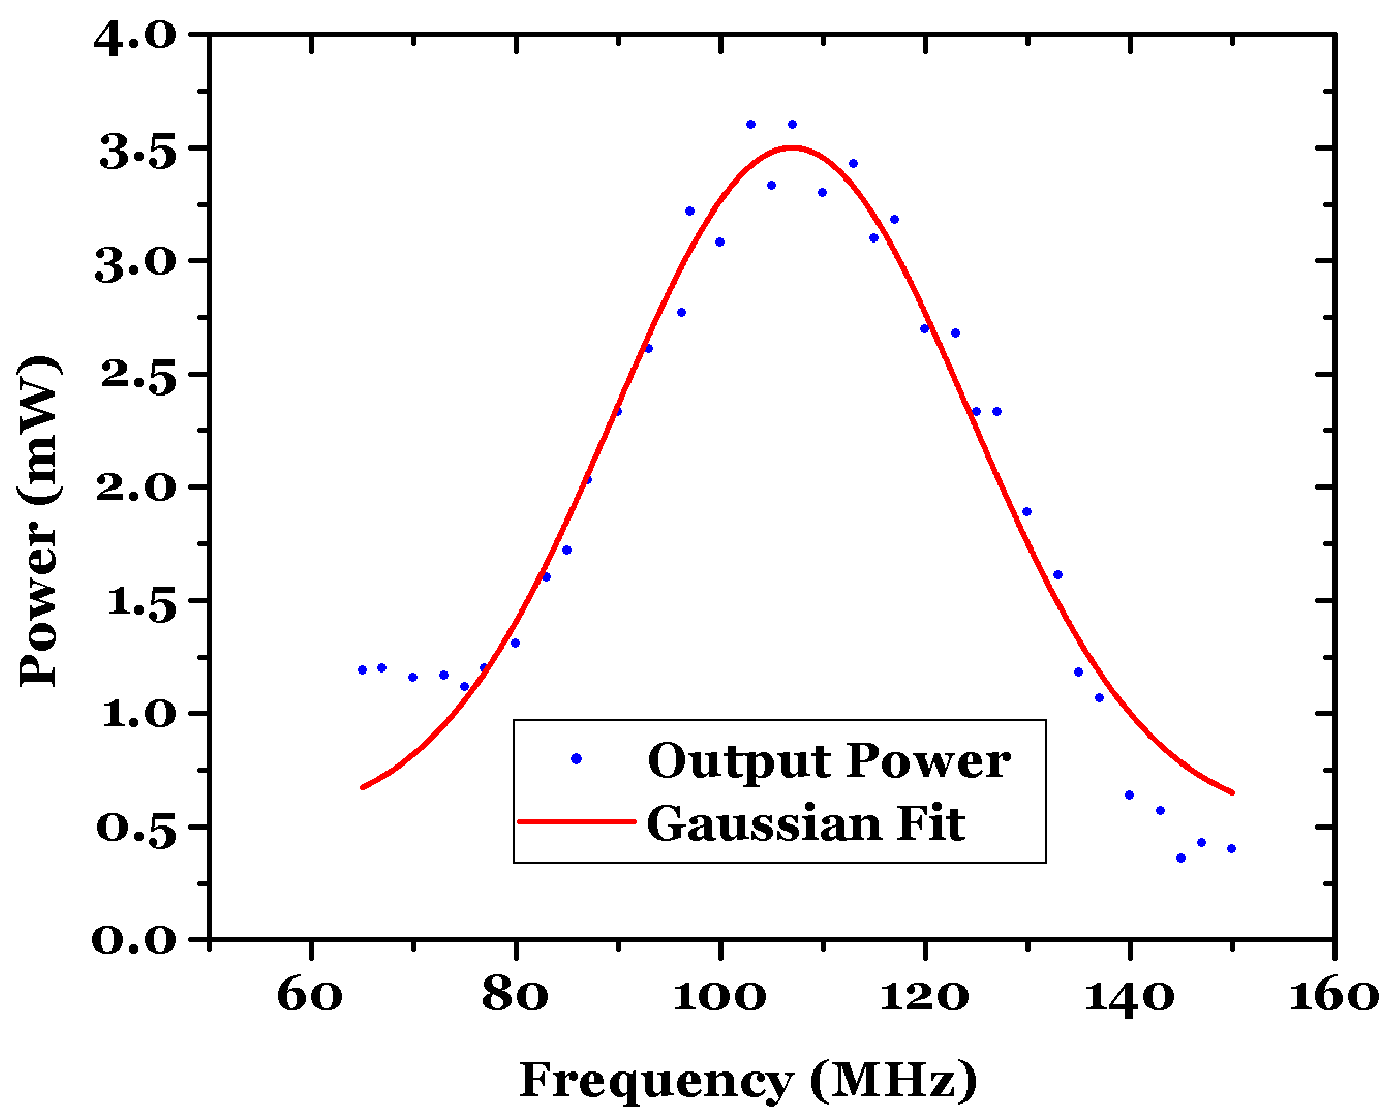
\includegraphics[height=2.5in]{figures/graph.png}
%
%    \caption[Optional: Short caption to appear in List of
%    Figures]{Full caption to appear below the Figure}
%
%    \label{figure1}
%\end{figure}

% +--------------------------------------------------------------------+
% |To create cross-references to figures, tables and segments
% |of text, LaTeX provides the following commands:
% |   \label{marker}
% |   \ref{marker}
% |   \pageref{marker}
% | where {marker} is a unique identifier.
% |
% | In the line above, we use \label{figure1} to mark a location
% | we wish to refer to later.  LATEX replaces \ref by the number of
% | the chapter, section, subsection, figure, or table after which the
% | corresponding \label command was issued. \pageref prints the page
% | number of the page where the \label command occurred.
% |
% +--------------------------------------------------------------------+

%See the file chapter1.tex for examples of the commands used to
%insert a figure or table, add a caption, etc.  Here is an example of
%a table:

%\begin{table}[ht]
%
%% +--------------------------------------------------------------------+
%% | We include the command \begin{center} to center the table
%% | horizontally on the page.  Note use of the command \end{center}
%% | to turn off centering after the table is defined.
%% +--------------------------------------------------------------------+
%    \begin{center}
%
%% +--------------------------------------------------------------------+
%% | The table is created with this command
%% |
%% | \begin{tabular}[pos]{table spec}
%% |
%% | The "pos" argument specifies the vertical position of the table
%% | relative to the baseline of the surrounding text.  Use t, b, or c
%% | to specify alignment at the top, bottom, or center.
%% |
%% | The "table spec" command defines the format of the table
%% |   l for a column of left-aligned text
%% |   r for a column of right-aligned text
%% |   c for centered text
%% |   p{width} for a column containing justified text with line breaks
%% |   | for a vertical line
%% |
%% |  In this example, the caption is made to appear above the table
%% |  by positioning the \caption command before the \begin{tabular
%% |  command. To position the caption below the table, insert the
%% |  \caption command after the \end{tabular} command.
%% +--------------------------------------------------------------------+
%    \caption{Caption to appear above the table}
%    \begin{tabular}[c]{|c|c|c|}
%        \hline
%        Column 1 Heading & Column 2 Heading & Column 3 Heading \\
%        \hline
%        Col 1 Row 1 & Col 2 Row 1 & Col 3 Row 1\\
%        Col 1 Row 2 & Col 2 Row 2 & Col 3 Row 2\\
%        Col 1 Row 3 & Col 2 Row 3 & Col 3 Row 3\\
%        \hline
%    \end{tabular}
%
%    \label{table1}
%   \end{center}
%\end{table}



% +--------------------------------------------------------------------+
% | Replace \section headings below with the title of your
% | subsections.  LaTeX will automatically number the subsections 1.1,
% | 1.2, 1.3, etc.
% +--------------------------------------------------------------------+

%\section{Making References to Figures or Tables}
%\label{makereference1.1}
%
%It is possible to create cross-references and hyperlinks to items or
%sections within your paper.  For example, here is a reference to
%Fig.~\ref{figure1} mentioned at the beginning of this chapter and a
%reference to the Table~\ref{table1}.
%
%\section{Making a Reference to a Chapter Subsection}
%\label{makereference1.2}
%
%In this section, we refer back to text mentioned in
%Section~\ref{makereference1.1} on page~\pageref{makereference1.1}.
%
%\section{Making a Citation}
%\label{makereference1.3}
%
%Here's an example of a citation to a single
%work.~\citep{CT:Weiner:1999} It's also possible to make multiple
%citations.~\citep{CT:Phillips:1985, ARP:Loy:1974}
%
%This template uses BibTeX to manage and format citations.  BibTeX is
%not the only way to create a bibliography within LaTeX, but it's
%generally considered to be the best option for long documents like a
%thesis or dissertation.~\citep{CT:Gould:1988}  There are a few more
%sample citations in this paragraph so you can see examples of how
%in-text references are made and how the bibliography is
%formatted.~\citep{ARP:Melinger:1991} See the file "BibTeX Guide.pdf"
%for information on how to use BibTeX.

\cleardoublepage

\chapter{Weighted Leibniz-type rules with applications to scattering properties of PDEs}
\label{makereference2}

In this chapter we discuss bilinear multiplier operators associated to Coifman-Meyer multipliers and Leibniz-type rules in the settings of weighted Triebel-Lizorkin and Besov spaces.  Additionally we obtain applications of these results to scattering properties of certain systems of parial differential equations. One of the main results in this chapter is in the setting of Triebel-Lizorkin spaces based in weighted Lebesgue spacs and Hardy spaces. It is as follows. 

\begin{theorem}\label{thm:CM:TL:B}  For $m \in \re,$ let $\sigma(\xi,\eta),$ $\xi,\eta\in\rn,$ be a Coifman-Meyer multiplier of order $m.$ Consider  $0 < p, p_1, p_2  \le \infty$  such that $\hcline$ and  $0 < q \leq \infty;$ let  $w_1,w_2\in A_\infty$ and set $w=w_1^{{p}/{p_1}} w_2^{{p}/{p_2}}.$ 
If $0 < p,p_1,p_2 < \infty$ and  $s > \tau_{p,q}(w),$  it holds that
\begin{equation}\label{KP:CM:TL}
\norm{T_\sigma(f,g)}{\tlw{p}{s}{q}{w}} \lesssim \norm{f}{\tlw{p_1}{s+m}{q}{w_1} } \norm{g}{H^{p_2}(w_2)} +  \norm{f}{H^{p_1}(w_1)}   \norm{g}{\tlw{p_2}{s+m}{q}{w_2} } \quad \forall f, g \in \swz.
\end{equation}
If $0< p, p_1,p_2\leq \infty$ and $s > \tau_p(w)$, it holds that
\begin{equation}\label{KP:CM:B}
\norm{T_\sigma(f,g)}{\besw{p}{s}{q}{w}} \lesssim \norm{f}{\besw{p_1}{s+m}{q}{w_1} } \norm{g}{H^{p_2}(w_2)} +  \norm{f}{H^{p_1}(w_1)}   \norm{g}{\besw{p_2}{s+m}{q}{w_2} } \quad \forall f, g \in \swz,
\end{equation}
where the Hardy spaces $H^{p_1}(w_1)$ and $H^{p_2}(w_2)$ must be replaced by $L^\infty$ if $p_1=\infty$ or $p_2=\infty,$ respectively.

If $w_1=w_2$ then different pairs of $p_1, p_2$ can be used on the right-hand sides of \eqref{KP:CM:TL} and \eqref{KP:CM:B}; moreover, if $w\in A_\infty,$ then 
\begin{equation}\label{KP:CM:TL2}
\norm{T_\sigma(f,g)}{\tlw{p}{s}{q}{w}} \lesssim \norm{f}{\tlw{p}{s+m}{q}{w} } \norm{g}{L^\infty} +  \norm{f}{L^\infty}   \norm{g}{\tlw{p}{s+m}{q}{w}} \quad \forall f, g \in \swz,
\end{equation}
where $0<p<\infty,$ $0<q\le\infty$ and $s>\tau_{p,q}(w).$
\end{theorem}

In the following sections the function spaces and multipliers used in the hypotheses are defined and discussed. We will then remark on corollaries to Theorem (\ref{thm:CM:TL:B}) and their connection to the Leibniz rules in the previous chapter.  theorem and the proof of Theorem (\ref{thm:CM:TL:B}). The proof is quite flexible and can be readily adapted to Triebel-Lizorkin and Besov spaces based in other function spaces. 

\section{Definitions}

\subsection{Coifman-Meyer Multipliers}

The symbols used in Theorem (\ref{thm:CM:TL:B}) and results later in this chapter are Coifman-Meyer multipliers. Such multipliers are defined as follows.

\begin{dfn}\label{CM_def}
For $m\in\rn$, a smooth function $\sigma = \sigma(\xi,\eta)$, $\xi,\eta\in\rn$, is a \textit{Coifman-Meyer multiplier} of order $m$ if for all multi-indices $\alpha,\beta\in\mathbb{N}^n_0$ there exists a positive constant $C_{\alpha,\beta}$ such that 
\begin{equation}\label{eq:CMm}
|\partial_\xi^\alpha \partial_\eta^\beta \sigma(\xi, \eta)| \leq C_{\alpha, \beta} (|\xi|+|\eta|)^{m -(\abs{\alpha}+ \abs{\beta})} \quad \forall (\xi, \eta) \in \re^{2n} \setminus \{(0,0)\}.
\end{equation}
\end{dfn}
Operators associated to these multipliers have been widely studied. For instance in Grafakos-Torres \cite{MR1880324} operators associated to Coifman-Meyer multipliers were studied because of their connection to a larger class of operators called Calder\'on-Zygmund operators. In particular it holds that 
\[ \norm{T_\sigma(f,g)}{L^p}\lesssim \norm{f}{L^{p_1}}\norm{g}{L^{p_2}} \]
where $\sigma$ is a Coifman-Meyer multiplier, $\frac{1}{p} = \frac{1}{p_1} + \frac{1}{p_2}$, and $1<p_1,p_2<\infty$. 
We also note that in particular Coifman-Meyer multipliers of order $m$ belong to the bilinear H\"ormander class $\dot{BS}^m_{1,1}$. These symbols and operators associated to them will be discussed in the following chapter. 
%% +--------------------------------------------------------------------+
% | Sample Chapter 3
% +--------------------------------------------------------------------+

\cleardoublepage

% +--------------------------------------------------------------------+
% | Replace "This is Chapter 3" below with the title of your chapter.
% | LaTeX will automatically number the chapters.                      
% +--------------------------------------------------------------------+

\chapter{Bilinear H\"ormander Classes of Critical Order}\label{chapter3}
\label{makereference3}

\section{Introduction}

In this chapter we obtain Leibniz-type rules for bilinear multiplier operators associated to symbols in the H\"ormander classes of critical order in the setting of local Hardy spaces. First, we will discuss the bilinear H\"ormander classes $BS^m_{\rho,\delta}$ and what it means for these symbols to be of critical order. Given $0\leq \delta \leq \rho \leq 1$ and $m\in\re$, a complex-valued function $\sigma = \sigma(x,\xi,\eta)$, $x,\xi,\eta \in \rn$, belongs to the bilinear H\"ormander class $BS^m_{\rho,\delta}$ if for any multiindices $\alpha,\beta,\gamma \in \mathbb{N}^n_0$ there exists a positive constant $C_{\alpha,\beta,\gamma}$ such that 
\begin{equation}\label{def:Bmrd}
|\partial_x^\alpha \partial_\xi^\beta \partial_\eta^\gamma \sigma(x, \xi, \eta)| \leq C_{\alpha, \beta, \gamma} (1+|\xi|+|\eta|)^{m +\delta \abs{\alpha}-\rho(\abs{\beta+\gamma})} \quad \forall x, \xi, \eta \in \rn.
\end{equation}
Then for any $\sigma \in BS^m_{\rho,\delta},$ the bilinear pseudodifferential operator $T_\sigma$ associated to $\sigma$ is defined as in \ref{psydo}. Boundedness properties of bilinear pseudodifferential operators with symbols
in the bilinear H\"ormander classes have been extensively studied in the settings of
Lebesgue and Hardy spaces; see B\'enyi-Bernicot-Maldonado-Naibo-Torres \citep{MR2660466}, B\'enyi-Chaffee-Naibo \citep{benyi2018strongly}, B\'enyi-Maldonado-Naibo-Torres \citep{MR1986065, MR2660466}, Brummer-Naibo \citep{MR3750234}, Herbert-Naibo \citep{MR3627725}, \citep{MR3211086}], Koezuka-Tomita \citep{MR3750316}, Michalowski-Rule-Staubach \citep{MR3165300}, Miyachi-Tomita
\citep{MR3179688, miyachi2018bilinear, miyachi2018bilinear2}, Naibo \cite{MR3393696, MR3411149}, Rodr\'iguez-L\'opez-Staubach \citep{MR3035059}, and the references therein. One fundamental aspect of the study of such symbols is their symbolic calculus for the transposes of operators associated to them. This was established in the works B\'enyi-Torres \citep{MR1986065} and B\'enyi-Maldonado-Naibo-Torres \citep{MR2660466}. Another important aspect of the study of these operators is their boundedness properties in a variety of function spaces. Operators associated to symbols in $BS^0_{1,0}$ can be realized as Calder\'on-Zygmund operators. As a consequence operators associated to symbols in $BS^0_{1,0}$ are bounded from $L^{p_1}(\rn) \times L^{p_2}(\rn)$ to  $L^p(\rn)$ for  $1 < p_1, p_2 < \infty$ and $1/2<p <\infty$ related through $\hcline.$ These operators also satisfy the endpoint mappings $L^\infty(\rn) \times L^\infty(\rn) \rightarrow BMO(\rn)$ and $L^1(\rn) \times L^1(\rn) \rightarrow L^{1/2, \infty}(\rn)$. For the development of the Calder\'on-Zygmund theory see Coifman-Meyer \citep{MR518170}, Kenig-Stein \citep{MR1713146}, and Grafakos-Torres \citep{MR1880324}. Operators with symbols in the forbidden class $BS^0_{1,1}$ may fail to be bounded in Lebesgue spaces. As such operators associated to these symbols are better understood in other settings. In B\'nyi et al. ~\cite{MR1996120, MR2250054, MR1986065} estimates in Sobolev spaces were obtained for such operators. For results in the settings of Besov and Triebel-Lizorkin spaces see Brummer--Naibo~\cite{MR3750234}, Koezuka--Tomita~\cite{MR3750316} and Naibo~\cite{MR3393696}.


Given  $0\le \delta\le \rho< 1$  and $0< p_1,p_2,p\le \infty$  related   by $\hcline,$ define 
$$
m(\rho, p_1,p_2):=-n(1-\rho)\max({1}/{2},\,{1}/{p_1},{1}/{p_2},\, 1-1/p, 1/p-1/2).
$$ 

B\'enyi et al.~\cite{MR3205530} proved that if $1\le p_1,p_2, p\le \infty,$    $m<m(\rho,p_1,p_2)$ and $\sigma\in BS^m_{\rho,\delta}$  then $T_\sigma$ is bounded from $L^{p_1}(\rn)\times L^{p_2}(\rn)$ to $L^p(\rn).$  On the other hand, Miyachi--Tomita~\cite{MR3179688} proved that  if $m>m(\rho, p_1,p_2),$ with $0< p_1,p_2,p\le \infty,$ there are symbols in $BS^m_{\rho,\rho}$ for which the associated  bilinear pseudodifferential operators are not bounded from $H^{p_1}(\rn)\times H^{p_2}(\rn)$ to $L^p(\rn)$ and therefore are not bounded from $L^{p_1}(\rn)\times L^{p_2}(\rn)$ to $L^p(\rn)$; recall that $H^{p}(w)(\rn)=L^p(w)(\rn)$ if $1<p<\infty)$ and $\norm{f}{H^p(w)} \leq \norm{f}{L^p(w)}$ when $0<p\leq 1$. In the case that $p=\infty$ $L^p(\rn)$ should be replaced by $BMO(\rn)$. Because of the two results stated above the class $BS^{m(\rho,p_1,p_2)}_{\rho,\delta}$ is referred to as a critical class and $m(\rho,p_1,p_2)$ is called a critical order. 

We now turn our attention to the critical classes. Miyachi--Tomita~\cite{MR3179688} showed that the symbols in $BS^{m(0,p_1,p_2)}_{0,0}$ with $0<p_1,p_2,p\le  \infty $ give rise to operators that are bounded from  $h^{p_1}(\rn)\times h^{p_2}(\rn)$ to $h^p(\rn),$ where $h^{r}(\rn)$ denotes a local Hardy space (recall that $h^{r}(\rn)=L^r(\rn)$ if $1<r<\infty$)  and $h^{r}(\rn)$ should be replaced with $bmo(\rn)$ if $r=\infty.$   In the case that $p_1 = p_2 = \infty$ Naibo~\cite{MR3411149}  proved  that if $\sigma$ is in the critical class $BS^{m(\rho, \infty,\infty)}_{\rho,\delta}$ with $0\le \delta\le \rho<1/2 $ then $T_\sigma$ is bounded from $L^{\infty}(\rn)\times L^{\infty}(\rn)$ to $BMO(\rn).$ Recently the theory of boundedness properties in the setting of Lebesgue and  Hardy  spaces for operators with symbols in the critical classes was completed in Miyachi--Tomita~\cite{MT1, MT2}: operators with symbols of critical order $ m(\rho, p_1,p_2),$ with $0\le \delta\le \rho<1$  and $0< p_1,p_2,p\le \infty,$ are bounded from $H^{p_1}(\rn)\times H^{p_2}(\rn)$ to $L^p(\rn),$ where  $L^p(\rn)$ should be replaced by $BMO(\rn)$ if $p=\infty.$

In this chapter we prove estimates in the setting of Besov and Hardy spaces for bilinear pseudodifferential operators associated to symbols in the critical classes $BS^{m(\rho,p_1,p_2)}_{\rho,\delta}$. The main result of this chapter is the following theorem.

\begin{theorem} \label{thm:main1}
Let $0<p<\infty$ and  $0<p_1,p_2\le \infty$ be such that $\hcline,$ $0<q\le \infty,$   $0\le\delta\le \rho<1$ and   $\sigma\in BS^{m(\rho,p_1,p_2)}_{\rho,\delta}.$ If $s>\text{max}(0,n(1/p - 1)),$ then it holds that
\begin{equation}\label{eq:main1}
\norm{T_\sigma(f,g)}{\ibes{p}{s}{q}}\lesssim \norm{f}{\ibes{p_1}{s}{q}}\norm{g}{h^{p_2}} +\norm{f}{h^{p_1}}\norm{g}{\ibes{p_2}{s}{q}}\quad \forall f,g\in \sw,
\end{equation}
where $h^{p_1}$ and $h^{p_2}$ must be replaced by $L^\infty$ if $p_1=\infty$ or $p_2=\infty,$ respectively. Moreover,  if there exits $\varepsilon>0$ such that the Fourier transform of  $\sigma(\cdot,\xi,\eta)$ is  supported outside the set  $\{\zeta\in\rn:\abs{\zeta}<\varepsilon (\abs{\xi}+\abs{\eta})\}$ for all  $\xi,\eta\in\rn$ such that $1/32\abs{\xi}\le \abs{\eta}\le 32 \abs{\eta},$ then \eqref{eq:main1} holds for any $s\in\re.$
\end{theorem}

Results related to estimate \ref{eq:main1} were proved for the forbidden class $BS^0_{1,1}$ in B\'enyi \cite{MR1996120}, Koezuka-Timita \cite{MR3750316}, and Naibo \citep{MR3393696}. Concerning bilinear pseudodifferential operators with symbols belonging to the subcritical classes $BS^m_{\rho,\delta}$ with $m<m(\rho,p_1,p_2)$ and $1\leq p_1,p_2,p \leq \infty$ ($1 < p_1,p_2,p < \infty$ when $\rho = \delta = 0$) estimate \ref{eq:main1} was shown in Naibo \citep{MR3393696} Theorem 1.3. Theorem \ref{thm:critical_besov} extends this result to the critical classes and allows for the indices to be in the wider range $(0,\infty)$. 

The proof of Theorem~\ref{thm:main1} uses the fact that operators with symbols in $BS^{(0,p_1,p_2)}_{0,0}$ that are localized at certain dyadic frequencies are bounded in the setting of local Hardy spaces; no other boundedness properties of operators with symbols in the bilinear H\"ormander classes are required in the proof. The tools employed are inspired by bilinear techniques in Naibo~\cite{MR3393696} and linear ones in   Johnsen~\cite{MR2163627}, Marschall~\cite{MR1376592} and   Park~\cite{MR3759556}.

As a consequence of Theorem~\ref{thm:main1}, we obtain  Leibniz-type rules for bilinear pseudodifferential operators associated to symbols in a general class $BS^m_{\rho,\delta}:$

\begin{corollary}\label{coro:main1} 
Let $0<p<\infty$ and $0<p_1,p_2\le \infty$ be such that $\hcline,$ $0<q\le \infty,$  $0\le\delta \le \rho<1,$   $m\in \re$ and $\sigma\in BS^{m}_{\rho,\delta};$ set $\bar{m}=m-m(\rho,p_1,p_2).$  If  $s>\max(0,n({1}/{p}-1))$ then it holds that
\begin{equation}\label{eq:coro:main1}
\norm{T_\sigma(f,g)}{\B{s}{p}{q}}\lesssim \norm{f}{\B{s+\bar{m}}{p_1}{q}}\norm{g}{h^{p_2}} +\norm{f}{h^{p_1}}\norm{g}{\B{s+\bar{m}}{p_2}{q}}\quad \forall f,g\in \sw,
\end{equation}
where $h^{p_1}$ and $h^{p_2}$ must be replaced by $L^\infty$ if $p_1=\infty$ or $p_2=\infty,$ respectively. Moreover,  if there exits $\varepsilon>0$ such that the Fourier transform of  $\sigma(\cdot,\xi,\eta)$ is  supported outside the set  $\{\zeta\in\rn:\abs{\zeta}<\varepsilon (\abs{\xi}+\abs{\eta})\}$ for all  $\xi,\eta\in\rn$ such that $1/32\abs{\xi}\le \abs{\eta}\le 32 \abs{\eta},$ then \eqref{eq:coro:main1} holds for any $s\in\re.$
\end{corollary}

\begin{remark} If $0\le \delta\le \rho<1,$ $m<m(\rho,p_1,p_2)$ and $\sigma\in BS^m_{\rho,\delta}$ then $T_\sigma$ is a smoothing operator since, in such case, $s+\bar{m}<s$ for $s,\bar{m}$ as in the statement of Corollary~\ref{coro:main1}. 
\end{remark}

\begin{remark} It will be clear from the proofs that different pairs of $p_1,p_2,$ related to $p$ through the H\"older condition, can be used in each of the terms on the right-hand sides of the estimates in Theorem~\ref{thm:main1} and Corollary~\ref{coro:main1}. 
\end{remark}

\section{Preliminaries}


\subsection{Marchall's inequality for bilinear pseudodiffernetial operators}
In this section we let the maximal function $\mathcal{M}_r$ be defined as in \ref{maximal_Mr}. Recall that by properties of the Hardy-Littlewood maximal function $\mathcal{M}$, it follows that if $r\leq p\leq \infty$ then 
\begin{equation}
\norm{\mathcal{M}_r(f)}{L^p} \lesssim \norm{f}{L^p}.
\end{equation}

The following result follows from   Marschall~\cite[p.118, Proposition 5(a)]{MR1376592} and  Johnsen~\cite[p.275, Proposition 4.1]{MR2163627}:

\begin{lem}\label{lem:Marschall} Consider $F\in \mathcal{S}(\re^N)$ and let $\Sigma=\Sigma(X, \zeta)$ be a  symbol in $C^\infty(\re^N \times \re^N)$ such that for some polynomial $P(\zeta),$
\[
\abs{\Sigma(X, \zeta)}\lesssim P(\zeta)\quad \forall X,\zeta\in\re^N.
\]
Suppose there exists $k_0\in \ent$ such that
$$
\supp (\Sigma(X, \cdot)) \subset  \{ \zeta \in \re^N:  |\zeta| \le 2^{k_0}\}\quad \forall X\in \re^N
$$
and
$$
\supp(\widehat{F})  \subset  \{ \zeta \in \re^N:  |\zeta| \le 2^{k_0}\}.
$$
If $0<r \le 1$ and $\norm{\Sigma(X, 2^{k_0} \cdot)}{\dot{B}^{N/r}_{1,r}(\re^N)} \mathcal{M}_r(F)(X)$ is locally integrable in $\re^N,$ it holds that
\begin{equation}\label{eq:Marschall:N}
|T_{\Sigma}(F)(X)| \lesssim \norm{\Sigma(X, 2^{k_0} \cdot)}{\dot{B}^{N/r}_{1,r}(\re^N)} \mathcal{M}_r(F)(X) \quad \forall X \in \re^N,
\end{equation}
where the implicit constant is independent of $\Sigma,$ $F$ and $k_0.$
\end{lem}

We will use Lemma \ref{lem:Marschall} to prove the following bilinear version of Marschall's inequality that is used in the proof of Theorem \ref{thm:main1}:
\begin{lemma}\label{lem:biMarschall}  Consider $f,g\in\sw$  and let $\sigma=\sigma(x,\xi,\eta)$ be a  symbol in $C^\infty(\re^{3n})$ 
such that for some polynomial $P(\xi,\eta),$
\[
\abs{\sigma(x,\xi,\eta)}\lesssim P(\xi,\eta)\quad \forall x,\xi,\eta\in\rn.
\]
Suppose there exists $k_0\in\ent$  such that
$$
\supp(\sigma(x, \cdot, \cdot)) \subset \{(\xi, \eta) \in \re^{2n}: |\xi| + |\eta| \le 2^{k_0}\}\quad \forall x\in\rn
$$
and 
$$
\supp(\widehat{f}), \supp(\widehat{g}) \subset \{\xi \in \re^{n}: |\xi| \le 2^{k_0}\}.
$$
If $0< r\le1$ and $\norm{\sigma(x, 2^{k_0+1} \cdot, 2^{k_0+1} \cdot)}{W^{\lfloor{2n/r}\rfloor + 1,1}(\re^{2n})} \mathcal{M}_r(f\otimes g)(x,y) $ is locally integrable in $\rtn,$ it holds that
\begin{equation}\label{eq:biMarschall}
|T_{\sigma}(f,g)(x)| \lesssim  \norm{\sigma(x, 2^{k_0+1} \cdot, 2^{k_0+1} \cdot)}{W^{\lfloor{2n/r}\rfloor + 1,1}(\re^{2n})} \mathcal{M}_r(f)(x) \mathcal{M}_r(g)(x) \quad \forall x \in \rn,
\end{equation}
where the implicit constant is independent of $\sigma,$  $f,$ $g$ and $k_0.$
\end{lemma}
\begin{proof}
 We have that
$$
T_{\sigma}(f,g)(x) = \int_{\rtn} \sigma(x, \xi, \eta) \fhat(\xi) \ghat(\eta) \eixxe\dxi\deta
$$
can be regarded as the restriction to the diagonal in $\re^{2n}$ of the linear pseudodifferential operator
$$
T_\Sigma(F)(X) = \int_{\re^{2n}} \Sigma(X, \zeta) \widehat{F}(\zeta) e^{2\pi i X \cdot \zeta } \dzeta
$$
after setting $\zeta=(\xi, \eta)$ and defining, for $X = (x, y) \in \re^{2n}$, 
$$
\Sigma(X, \zeta) :=\sigma(x, \xi, \eta)\quad and \quad F(X):= (f\otimes g) (X)=f(x)g(y).
$$
Note that $\Sigma(X, \zeta)$ is in $C^\infty(\rtn\times \rtn),$  has polynomial growth in $\zeta$ uniformly in $X$ and  is supported in $\{\zeta\in\re^{2n}: \abs{\zeta}\le 2^{k_0}\}$ for each $X\in \rtn;$ moreover $\widehat{F}(\zeta) =  \widehat{f}(\xi) \widehat{g}(\eta)$ is supported in $\{\zeta \in \re^{2n}: |\zeta| \leq 2^{k_0+1} \}.$ Then, \eqref{eq:biMarschall} follows after applying Lemma~\ref{lem:Marschall}  and \eqref{eq:Marschall:N:Sob} to $T_{\Sigma}(F)$ and noticing that 
\[
\mathcal{M}_r(F)(x, x)\lesssim \mathcal{M}_r(f)(x)\mathcal{M}_r(g)(x)\quad \forall x\in\rn.
\]
\end{proof}

\begin{remark}
We note that $\norm{\sigma(x, 2^{k_0+1} \cdot, 2^{k_0+1} \cdot)}{W^{\lfloor{2n/r}\rfloor + 1,1}(\re^{2n})} \mathcal{M}_r(f\otimes g)(x,y) $ is locally integrable when  $\norm{\sigma(x, 2^{k_0+1} \cdot, 2^{k_0+1} \cdot)}{W^{\lfloor{2n/r}\rfloor + 1,1}(\re^{2n})}$ is a bounded function of $x$ since $\mathcal{M}_r(f\otimes g)(x,y)$ is locally integrable.
\end{remark}


\section{Decomposition of $T_\sigma$ and strategy for the proof of Theorem \ref{thm:main1}}\label{sec:decomp}
In the proofs that follow in this chapter we implicitly assume that the symbol $\sigma$ in the statements of Theorem \ref{thm:main1} and Corollary \ref{coro:main1} has compact support in $\mathbb{R}^{3n}$. A limiting argument then allows us to to prove these results for sumbols in the bilinear H\"ormander classes without compact support. For $0\le \delta,\rho\le 1,$ $m\in\re,$ $\sigma\in BS^m_{\rho,\delta}$ and $0\le \varepsilon<1$ let $\sigma_\epsilon (x,\xi,\eta) = \Psi(\varepsilon x, \varepsilon \xi, \varepsilon \eta) \sigma( x, \xi,\eta)$ for a smooth  function $\Psi$ of compact support such that $\Psi(0,0,0) = 1$. It follows that $\sigma_\varepsilon \in BS^m_{\rho,\delta}$ with constants independent of $\varepsilon$ and that, as $\varepsilon \rightarrow 0$, $T_{\sigma_\varepsilon}(f,g)$ converges to $T_\sigma(f,g)$ in $\swp$ for $f,g \in \sw$. Indeed, using the smoothness and compact support of $\Psi$ and the Leibniz rule we have that 
\begin{align*}
|\partial^\alpha_\xi \partial^\beta_\eta \sigma_\varepsilon(x,\xi,\eta)| & 
\leq \sum_{\alpha_0 \leq \alpha, \beta_0 \leq \beta} \varepsilon^{|\alpha_0| + |\beta_0|}|\partial^{\alpha_0}_\xi \partial^{\beta_0}_\eta \Psi(\varepsilon x, \varepsilon \xi, \varepsilon \eta) \partial^{\alpha - \alpha_0}_\xi \partial^{\beta - \beta_0}_\eta \sigma(x,\xi,\eta) | \\
& \leq \sum_{\alpha_0 \leq \alpha, \beta_0 \leq \beta} C_{\alpha_0 , \beta_0} (1 + |\xi| + |\eta|)^{m + \delta|\alpha - \alpha_0| - \rho|\beta - \beta_0|} \\
& =(1 + |\xi| + |\eta|)^{m + \delta|\alpha| - \rho|\beta|} \sum_{\alpha_0 \leq \alpha, \beta_0 \leq \beta} C_{\alpha_0 , \beta_0} (1 + |\xi| + |\eta|)^{-\delta| \alpha_0| + \rho|\beta_0|} \\
& \leq C_{\alpha,\beta} (1 + |\xi| + |\eta|)^{m + \delta|\alpha| - \rho|\beta|},
\end{align*}
for $(x,\xi,\eta) \in \text{supp}(\Psi)$ and $\sigma_\varepsilon \in BS^m_{\rho,\delta}$. Additionally by the dominated convergence theorem and using that  $\Psi(0,0,0) = 1$ we get that $T_{\sigma_\eps}(f,g) \rightarrow T_\sigma(f,g)$ in $\swp$ as $\eps \rightarrow 0$. Finally by the Fatou property of Besov spaces the estimates for $T_\sigma$ follow from the estimates for $T_{\sigma_\eps}$ which are uniform in $\eps$. 

We now present the decomposition of $T_\sigma$ that will be used in the proof of Theorem \ref{thm:main1}. Let $\varphi,\varphi_0 \in \sw$ satisfy conditions \ref{TL_B_psi1} and \ref{TL_B_phi1} respectively, and be such that $\sumkNz \fk \equiv 1,$ where $\fk(\xi)=\f(2^{-k}\xi)$ for $\xi\in\rn$ and $k\in\na.$

Let $m \in \re,$ $0 \leq \delta\le \rho < 1$ and $\sigma \in BS^m_{\rho, \delta}.$  We perform a spectral decomposition of $T_\sigma(f,g)$ with $f,g\in\sw:$
\begin{align*}
T_\sigma(f,g)(x)&= \int_{\rtn} \sigma(x, \xi, \eta) \fhat(\xi) \ghat(\eta) \eixxe \dxi \deta \\
& =  \sumjkNz \int_{\rtn} \left( \int_{\rn} \widehat{\sigma}^1(\zeta, \xi, \eta) \eixzeta  d\zeta \right) \fk(\xi) \fj(\eta) \fhat(\xi) \ghat(\eta) \eixxe \dxi \deta\\
& =  \sum_{j,k,\ell\in\na_0} \left( \int_{\rn} \f_\ell(\zeta)\widehat{\sigma}^1(\zeta, \xi, \eta) \eixzeta  d\zeta \right) \fk(\xi) \fj(\eta) \fhat(\xi) \ghat(\eta) \eixxe \dxi \deta\\
&= \sum_{j,k,\ell\in\na_0}  T_{\sigma_{j,k,\ell}}(f,g)(x),
\end{align*}
where for $j,k, \ell \in \naz$ we define
\begin{equation*}
\sigma_{j,k,\ell}(x, \xi, \eta)= \fk(\xi) \fj(\eta) \int_{\rn}  \f_\ell(\zeta) \widehat{\sigma}^1(\zeta, \xi, \eta) \eixzeta  \dzeta.
\end{equation*}
Using this decomposition we define the following symbols

\begin{align*}
& \sigma^1:= \quad \sum\limits_{\ell=4}^\infty \sum\limits_{k=0}^{\ell - 4} \sum\limits_{j =0}^{k} \sigma_{j,k,\ell}, \quad \sigma^2:= \quad \sum\limits_{k=0}^\infty \sum\limits_{j=0}^k \sum\limits_{\ell =\max(0,k-3)}^{k+3} \sigma_{j,k,\ell},\quad\sigma^3:= \quad \sum\limits_{k=4}^\infty \sum\limits_{j=0}^k \sum\limits_{\ell =0}^{k-4} \sigma_{j,k,\ell},\\
&\sigma^4:= \quad \sum\limits_{\ell=5}^\infty \sum\limits_{j=1}^{\ell - 4} \sum\limits_{k =0}^{j-1} \sigma_{j,k,\ell}, \quad \sigma^5:= \quad  \sum\limits_{j=1}^\infty \sum\limits_{k=0}^{j-1} \sum\limits_{\ell =\max(0,j-4)}^{j+3} \sigma_{j,k,\ell},\quad \sigma^6:= \quad \sum\limits_{j=5}^\infty \sum\limits_{k=0}^{j-1} \sum\limits_{\ell =0}^{j-5} \sigma_{j,k,\ell},
\end{align*}
so that $\sigma = \sigma^1+\sigma^2+\sigma^3+\sigma^4+\sigma^5+\sigma^6.$ Notice that since $j\leq k$ in $\sigma_1$, $\sigma_2$, and $\sigma_3$ they are supported on the set $\{(x,\xi,\eta) \in \mathbb{R}^{3n} : |\eta| \leq 4|\xi|\}$. On the other hand $\sigma_4$, $\sigma_5$, and $\sigma_6$ are supported on $\{(x,\xi,\eta) \in \mathbb{R}^{3n} : |\xi| \leq 2|\eta|\}$. By taking the Fourier transform with respect to $x$ we have that $\widehat{\sigma^1(\cdot,\xi,\eta)}$ is supported on $\{\zeta\in\rn: \abs{\xi}\lesssim \abs{\zeta}\},$
$\widehat{\sigma^2(\cdot,\xi,\eta)}$ is supported on $\{\zeta\in\rn: \abs{\xi}\sim \abs{\zeta}\}$ and $\widehat{\sigma^3(\cdot,\xi,\eta)}$ is supported on $\{\zeta\in\rn: \abs{\zeta}\lesssim \abs{\xi}\}$. The supports of $\widehat{\sigma^4(\cdot,\xi,\eta)}$, $\widehat{\sigma^5(\cdot,\xi,\eta)}$, and $\widehat{\sigma^6(\cdot,\xi,\eta)}$ are in supported in similar sets with $|\xi|$ replaced by $|\eta|$. The proof of Theorem \ref{thm:main1} will follow from obtaining bounds for $T_{\sigma^j}$, $j=1,2,3,4,5,6$. In this dissertation we will show the proofs of the results for $T_{\sigma^1}$, $T_{\sigma^2}$, and $T_{\sigma^3}$. By symmetry the results for $T_{\sigma^4}$, $T_{\sigma^5}$, and $T_{\sigma^6}$ are obtained in an analogous way as $T_{\sigma^1}$, $T_{\sigma^2}$, and $T_{\sigma^3}$ respectively with the roles of $\xi$ and $\eta$ reversed.

In the proofs of Theorem \ref{thm:main1} and Corollary \ref{coro:main1} we will use the fact that $BS^m_{\rho,\delta}\subset BS^m_{\rho,\rho}$ for $m\in\re$ and $0\le \delta\le \rho\le 1$. With this in mind we will assume that $\rho = \delta$ in the proofs.

\subsection{Estimates for $T_{\sigma^1}$}
In this section we prove the estimates for the operator $T_{\sigma_1}$. First, we introduce some notation that will be used in the proof. 
For $\{\fk\}_{k\in\naz}$ as in Section~\ref{sec:decomp} we set
\begin{equation*}
\Phi_k(\xi):= \sum_{j=0}^k \varphi_j(\xi)=\f_0(2^{-k}\xi)\quad \forall \xi\in\rn, k\in\naz,
\end{equation*}
and consider $\widetilde{\f},\widetilde{\f}_0\in\sw$ satisfying conditions \ref{{TL_B_psi1} - \ref{TL_B_phi2}, respectively, and such that $\widetilde{\f}_0\f_0=\f_0$ and $\widetilde{\f}\f=\f.$ We then define $\widetilde{\f}_k(\xi)=\widetilde{\f}(2^{-k}\xi)$ for $\xi\in\rn$ and $k\in\na$ and $\widetilde{\Phi}_k(\xi)=\widetilde{\f}_0(2^{-k}\xi)$ for $\xi\in\rn$ and $k\in\naz.$ It holds that $\widetilde{\f}_k \fk = \fk$ and $\widetilde{\Phi}_k \Phi_k = \Phi_k$ for all $k\in\naz.$

The precise bounds for $T_{\sigma^1}$ are stated in the following lemma.

\begin{lemma}\label{lem:T1} Let $m \in \re,$  $0 \le \delta\le  \rho < 1$ and $\sigma \in BS^m_{\rho, \delta}$. If   $0<p,p_1,p_2\le \infty$ are such that $\hcline,$ $0 < q ,\bar{q}\leq \infty,$ $s_1, s_2 \in \re$, it holds that
\begin{equation}\label{eq:estT1}
\norm{T_{\sigma^1}(f,g)}{\ibes{s_1}{q}{p}}  \lesssim \norm{f}{\ibes{s_2}{p_1}{\bar{q}}} \norm{g}{h^{p_2}} \quad \forall f, g \in \sw,
\end{equation}
where $\sigma^1$ is as in Section~\ref{sec:decomp} and $h^{p_2}$ must be replaced by $L^\infty$ if $p_2=\infty.$
\end{lemma}


We note that in Lemma \ref{lem:T1} there is no restriction on the order $m$ of the symbol and the regularity indices, $s_1$ and $s_2$, can be different. In the case that $s=s_1=s_2$ Lemma \ref{lem:T1} implies the following estimate that is needed for the proof of Theorem \ref{thm:main1} 
$$\norm{T_{\sigma^1}(f,g)}{\ibes{p}{s}{q}}  \lesssim \norm{f}{\ibes{p_1}{s}{q}} \norm{g}{h^{p_2}} \quad \forall f, g \in \sw,$$
for $s\in\re$ and $\sigma\in BS^{m(\rho,p_1,p_2)}_{\rho,\delta}$.



\begin{proof}  Let $m,$ $\rho,$ $p,$ $p_1,$ $p_2,$ $q,$ $\bar{q},$ $s_1,$  $s_2,$ $\sigma,$ $\sigma^1,$ $f$ and $g$ be as in the statement of the lemma. 

For $\ell \in \naz$  set
$$
\sigma^1_\ell:=  \sum\limits_{k=0}^{\ell -4} \sum\limits_{j =0}^{k} \sigma_{j,k,\ell},
$$
so that $T_{\sigma^1}(f,g)= \sum\limits_{\ell=4}^\infty T_{\sigma^1_\ell}(f,g)$. Recalling the definition of $\Phi_k$ and $\sigma_{j,k,\ell},$ we have
\begin{align*}
T_{\sigma^1_\ell}(f,g)(x)= \int_{\re^{3n}} \sum\limits_{k=0}^{\ell -4}   \fk(\xi) \Phi_k(\eta)  \f_\ell(\zeta) \widehat{\sigma}^1(\zeta, \xi, \eta) \widehat{f}(\xi) \widehat{g}(\eta) e^{2\pi i x \cdot (\xi + \eta + \zeta)}  \dzeta \dxi \deta,
\end{align*}
and changing variables, we get
\begin{align*}
T_{\sigma^1_\ell}(f,g)(x)= \int_{\rn} \left( \int_{\rtn}  \sum\limits_{k=0}^{\ell -4}   \fk(\xi) \Phi_k(\eta)  \f_\ell(\omega- \xi - \eta) \widehat{\sigma}^1(\omega- \xi - \eta, \xi, \eta) \widehat{f}(\xi) \widehat{g}(\eta) \dxi \deta \right)  e^{2\pi i x \cdot \omega} \, d\omega.
\end{align*}
This yields
\begin{align*}
\widehat{T_{\sigma^1_\ell}(f,g)}(\omega)=  \int_{\rtn}  \sum\limits_{k=0}^{\ell -4}   \fk(\xi) \Phi_k(\eta)  \f_\ell(\omega- \xi - \eta) \widehat{\sigma}^1(\omega- \xi - \eta, \xi, \eta) \widehat{f}(\xi) \widehat{g}(\eta) \dxi \deta,
\end{align*}
where the integral effectively takes place when $ 2^{\ell-1}\le |\omega- \xi - \eta| \leq 2^{\ell +1}$ (keep in mind that $\ell\ge 4$)  as well as $|\xi| \leq 2^{\ell-3}$ and $|\eta| \leq 2^{\ell-3}.$  Consequently,
$\widehat{T_{\sigma^1_\ell}(f,g)}$ is supported in $\{\omega\in\rn: 2^{\ell-2}\le |\omega| \leq 2^{\ell +2}\}$. Then, the fact that  $T_{\sigma^1}(f,g)= \sum\limits_{\ell=4}^\infty T_{\sigma^1_\ell}(f,g)$  and  Lemma~\ref{lem:nikol} give
\begin{equation}\label{eq:T:sigma:1:fg}
\norm{T_{\sigma^1}(f,g)}{\B{s_1}{p}{q}} \lesssim  \left( \sum\limits_{\ell=4}^\infty 2^{\ell s_1q} \norm{T_{\sigma^1_\ell}(f,g)}{{L^p}}^q \right)^\frac{1}{q}.
\end{equation}

Recalling the definitions of $\widetilde{\f}_k$ and $\widetilde{\Phi}_k,$  we have
\begin{align*}
T_{\sigma^1_\ell}(f,g)(x) = 
  \sum\limits_{k=0}^{\ell -4} T_{\sigma^1_{\ell,k}}(\Delta^{\widetilde{\f}}_k f,\Delta^{\widetilde{\Phi}}_k g)(x),
\end{align*}
where, for each $k$ between $0$ and $\ell -4$, we set 
$$
\sigma^1_{\ell, k}(x, \xi, \eta):=\left( \int_{\rn}  \f_\ell(\zeta) \widehat{\sigma}^1(\zeta, \xi, \eta) e^{2\pi i x \cdot \zeta}  \dzeta \right)  \fk(\xi) \Phi_k(\eta).
$$ 
Since $\sigma^1_{\ell,k}$ satisfies 
$$\abs{\sigma^1_{\ell,k}(x,\xi,\eta)}\lesssim (1+\abs{\xi}+\abs{\eta})^m\quad \forall x,\xi,\eta\in\rn,$$
$\sigma^1_{\ell, k}(x,\cdot,\cdot)$ is supported on $\{(\xi, \eta) \in \re^{2n} : |\xi| + |\eta| \leq 2^{k+2}\}$ for all $x\in\rn$ and $\Delta^{\widetilde{\f}}_k f$ and $\Delta^{\widetilde{\Phi}}_k g$ are Schwartz functions with  Fourier transforms  supported in $\{\xi \in \rn: |\xi| \le 2^{k+1}\},$  we can apply the bilinear Marschall inequality \eqref{eq:biMarschall} with $0<r\le 1$ to get 
\begin{align}\label{eq:bound:h1:ell:k}
&|T_{\sigma^1_{\ell,k}}(\Delta^{\widetilde{\f}}_k f,
\Delta^{\widetilde{\Phi}}_k g)(x)| \\
&\hspace{0.5cm}\lesssim  \norm{\sigma^1_{\ell, k}(x, 2^{k+3} \cdot, 2^{k+3} \cdot)}{W^{\lfloor{2n/r}\rfloor + 1,1}(\re^{2n})} \mathcal{M}_r(\Delta^{\widetilde{\f}}_k f)(x)\mathcal{M}_r(
\Delta^{\widetilde{\Phi}}_k g)(x)\quad \forall x\in\rn.\nonumber
\end{align}
(See Remark~\ref{remark:locint} along with \eqref{eq:estsigkl} below.)

We next estimate $\norm{\sigma^1_{\ell, k}(x, 2^{k+3} \cdot, 2^{k+3} \cdot)}{W^{\lfloor{2n/r}\rfloor + 1,1}(\re^{2n})}.$ For ease of notation we just work with $2^k$ instead of $2^{k+3}.$ Notice that 
\begin{equation*}
\sigma^1_{\ell, k}(x, 2^k \xi, 2^k \eta) = \f(\xi) \f_0(\eta) \int_{\rn} \widecheck{\f_\ell}(y) \sigma(x-y, 2^k \xi, 2^k \eta)\dy\quad \forall k\in\na,
\end{equation*}
with a similar expression for $\sigma^1_{\ell, 0}$ obtained by replacing $\f$ with $\f_0$ in the formula above. 
 For $\ell \geq 4$ the function $\widecheck{\f_\ell}$ has vanishing moments of every order; if $N \in \na$, we can then write
\begin{align*}
 I_{\ell, k}(\xi, \eta)&:= \int_{\rn} \widecheck{\f_\ell}(y) \sigma(x-y, 2^k \xi, 2^k \eta)\dy=2^{n \ell}\int_{\rn} \widecheck{\f}(2^{\ell}y) \sigma(x-y, 2^k \xi, 2^k \eta)\dy\\
& = 2^{n \ell} \int_{\rn} \widecheck{\f}(2^{\ell}y) \left( \sigma(x-y, 2^k \xi, 2^k \eta) - \sum\limits_{|\alpha| < N} \frac{1}{\alpha!} (-y)^\alpha \partial_x^\alpha \sigma(x, 2^k \xi, 2^k \eta) \right)\dy\\
& = 2^{n \ell} \int_{\rn} \widecheck{\f}(2^{\ell}y) \sum\limits_{|\alpha| = N} \frac{N}{\alpha!} (-y)^\alpha \int_0^1 (1-t)^{N-1} \partial_x^\alpha \sigma(x - t y, 2^k \xi, 2^k \eta) \dy.
\end{align*}
Given multiindices $\beta, \gamma \in \naz^n$ and using that $\sigma \in BS^m_{\rho, \rho}$, it follows that
\begin{align*}
& |\partial_\xi^{\beta} \partial_\eta^{\gamma}  I_{\ell, k}(\xi, \eta)|\\
& = 2^{n \ell} 2^{k (|\beta+ \gamma|)}  \left|  \int_{\rn} \widecheck{\f}(2^{\ell}y) \sum\limits_{|\alpha| = N} \frac{N}{\alpha!} (-y)^\alpha \int_0^1 (1-t)^{N-1} \partial_x^\alpha \partial_\xi^{\beta} \partial_\eta^{\gamma}\sigma(x - t y, 2^k \xi, 2^k \eta) \,dt\dy \right|\\
& \lesssim  2^{k (|\beta+ \gamma|)}  (1+ |2^k \xi| + |2^k \eta|)^{m + \rho N -  \rho|\beta+ \gamma|} \int_{\rn} 2^{n \ell} |\widecheck{\f}(2^{\ell}y)| |y|^N \dy \\
&\lesssim 2^{- N \ell} 2^{k (|\beta+ \gamma|)}  (1+ |2^k \xi| + |2^k \eta|)^{m + \rho N -  \rho |\beta+ \gamma|}.
\end{align*}
Then, for $(\xi,\eta)$ in the support of $\sigma^1_{\ell,k}(x, 2^k\cdot,2^k\cdot)$  we get
\begin{equation*}
 |\partial_\xi^{\beta} \partial_\eta^{\gamma}  I_{\ell, k}(\xi, \eta)| \lesssim 2^{- N \ell} 2^{k (1-\rho)|\beta+ \gamma|} 2^{k (m+\rho N)}.
\end{equation*}
Given $0< r \le 1$, taking  derivatives up to order $\lfloor{2n/r}\rfloor + 1$ in $(\xi,\eta)$ of
$\sigma^1_{\ell, k}(x, 2^k \xi, 2^k \eta) = \f(\xi) \f_0(\eta)  I_{\ell, k}(\xi, \eta),$
 we obtain
\begin{align}\label{eq:estsigkl}
  \norm{\sigma^1_{\ell, k}(x, 2^{k} \cdot, 2^{k} \cdot)}{W^{\lfloor{2n/r}\rfloor + 1,1}(\re^{2n})} \lesssim 2^{- N \ell} 2^{k (1-\rho)( \lfloor{2n/r}\rfloor + 1)} 2^{k (m+\rho N)}.
\end{align}
From \eqref{eq:bound:h1:ell:k}, it then follows that for all $x\in\rn,$ we have
\begin{equation*}
|T_{\sigma^1_{\ell,k}}(\Delta^{\widetilde{\f}}_k f,\Delta^{\widetilde{\Phi}}_k g)(x)|  \lesssim 2^{- N \ell} 2^{k [(1-\rho)( \lfloor{2n/r}\rfloor + 1)+m+\rho N]}    \mathcal{M}_r(\Delta{\widetilde{\f}}_k f)(x)\mathcal{M}_r(\Delta^{\widetilde{\Phi}}_k g)(x).
\end{equation*}

  Define $\pst=\min(1,p).$  For the sake of notation, we will next work with $q$ finite; the case $q=\infty$ can be treated analogously.
  Recalling that $T_{\sigma^1_\ell}(f,g)= \sum\limits_{k=0}^{\ell -4} T_{\sigma^1_{\ell,k}}(\Delta^{\widetilde{\f}}_k f,\Delta^{\widetilde{\Phi}}_k g)$,  \eqref{eq:T:sigma:1:fg} and the last  estimate give
\begin{align}
& \norm{T_{\sigma^1}(f,g)}{\B{s_1}{p}{q}}  \lesssim  \left( \sum\limits_{\ell=4}^\infty 2^{\ell s_1q} \norm{T_{\sigma^1_\ell}(f,g)}{L^p}^q \right)^\frac{1}{q}\label{eq:T1:fg:Fqp}\\
& \lesssim  \left[  \sum\limits_{\ell=4}^\infty 2^{\ell s_1 q} \left(  \sum\limits_{k=0}^{\ell -4} 2^{- N\pst \ell} 2^{k\pst [(1-\rho)( \lfloor{2n/r}\rfloor + 1)+m+\rho N]}   \norm{\mathcal{M}_r(\Delta^{\widetilde{\f}}_kf)\mathcal{M}_r(\Delta^{\widetilde{\Phi}}_k g)}{L^p}^{\pst}\right)^\frac{q}{\pst} \right]^\frac{1}{q}. \nonumber
\end{align}
Next, let us see that, for  $N>s_1$ and $0<\epsilon< N-s_1,$  it holds that
\begin{align}\nonumber
& \sum\limits_{\ell=4}^\infty 2^{\ell  s_1 q} \left(  \sum\limits_{k=0}^{\ell -4} 2^{- N \pst\ell} 2^{k \pst[(1-\rho)( \lfloor{2n/r}\rfloor + 1)+m+\rho N]}    \norm{\mathcal{M}_r(\Delta^{\widetilde{\f}}_k f)\mathcal{M}_r(\Delta^{\widetilde{\Phi}}_kg)}{L^p}^{\pst}\right)^{\frac{q}{\pst}} \\ \label{eq:moving:the:sums}
&\hspace{2cm}\lesssim \sum\limits_{k=0}^\infty 2^{k q[ (1-\rho)( \lfloor{2n/r}\rfloor + 1-N) + m+ s_1+\eps] }   \norm{\mathcal{M}_r(\Delta^{\widetilde{\f}}_k f)\mathcal{M}_r(\Delta^{\widetilde{\Phi}}_k g)}{L^p}^q.
\end{align}
 Indeed, if $0 < q \leq \pst$, we have
\begin{align*}
& \sum\limits_{\ell=4}^\infty  2^{\ell  s_1 q} \left(  \sum\limits_{k=0}^{\ell -4} 2^{- N \pst \ell} 2^{k \pst [(1-\rho)( \lfloor{2n/r}\rfloor + 1)+m+\rho N]}   \norm{\mathcal{M}_r(\Delta^{\widetilde{\f}}_k f)\mathcal{M}_r(\Delta^{\widetilde{\Phi}}_k g)}{L^p}^{\pst}\right)^\frac{q}{\pst} \\
& \leq \sum\limits_{\ell=4}^\infty 2^{-(N-s_1) q \ell} \sum\limits_{k=0}^{\ell -4}  2^{k q [(1-\rho)( \lfloor{2n/r}\rfloor + 1) + m+\rho N]}   \norm{\mathcal{M}_r(\Delta^{\widetilde{\f}}_k f)\mathcal{M}_r\Delta^{\widetilde{\Phi}}_k g)}{L^p}^q\\
&= \sum_{k=0}^{\infty} \left(\sum_{\ell=k+4}^\infty 2^{-(N-s_1) q \ell} \right)  2^{k q [(1-\rho)( \lfloor{2n/r}\rfloor + 1) + m+\rho N]}   \norm{\mathcal{M}_r(\Delta^{\widetilde{\f}}_k f)\mathcal{M}_r(\Delta^{\widetilde{\Phi}}_k g)}{L^p}^q \\
& \lesssim \sum\limits_{k=0}^\infty  2^{k q [(1-\rho)( \lfloor{2n/r}\rfloor + 1) + m+\rho N]} 2^{-kq(N-s_1)}   \norm{\mathcal{M}_r(\Delta^{\widetilde{\f}}_k f)\mathcal{M}_r(\Delta^{\widetilde{\Phi}}_k g)}{L^p}^q,
\end{align*}
and \eqref{eq:moving:the:sums} follows for any $\eps>0.$ Now, if $\pst<q <\infty$ and $0<\eps < N - s_1,$ we have
\begin{align*}
& \sum\limits_{\ell=4}^\infty   2^{\ell  s_1 q} \left(  \sum\limits_{k=0}^{\ell -4} 2^{- N \pst \ell} 2^{k \pst [(1-\rho)( \lfloor{2n/r}\rfloor + 1) +m+\rho N]}   \norm{\mathcal{M}_r(\Delta^{\widetilde{\f}}_k f)\mathcal{M}_r(\Delta^{\widetilde{\Phi}}_k g)}{L^p}^{\pst}\right)^\frac{q}{\pst} \\
& \lesssim \sum\limits_{\ell=4}^\infty 2^{-  (N- s_1 - \eps) q \ell}  \left(  \sum\limits_{k=0}^{\ell -4} 2^{-\eps \pst k} 2^{k \pst [(1-\rho)( \lfloor{2n/r}\rfloor + 1) + m+\rho N]}   \norm{\mathcal{M}_r(\Delta^{\widetilde{\f}}_k f)\mathcal{M}_r(\Delta^{\widetilde{\Phi}}_k g)}{L^p}^{\pst}\right)^\frac{q}{\pst}\\
& \lesssim  \sum\limits_{\ell=4}^\infty 2^{-  (N- s_1 - \eps) q \ell} \sum\limits_{k=0}^{\ell -4} 2^{k q [(1-\rho)( \lfloor{2n/r}\rfloor + 1) + m+\rho N]}   \norm{\mathcal{M}_r(\Delta^{\widetilde{\f}}_k f)\mathcal{M}_r(\Delta^{\widetilde{\Phi}}_k g)}{L^p}^q \\
& =  \sum\limits_{k=0}^\infty \left( \sum\limits_{\ell=k+4}^{\infty} 2^{- (N- s_1 - \eps) q \ell} \right) 2^{k q [(1-\rho)( \lfloor{2n/r}\rfloor + 1) + m+\rho N]}   \norm{\mathcal{M}_r(\Delta^{\widetilde{\f}}_k f)\mathcal{M}_r(\Delta^{\widetilde{\Phi}}_k g)}{L^p}^q \\
& \lesssim \sum\limits_{k=0}^\infty  2^{- (N- s_1 - \eps) kq } 2^{k q [(1-\rho)( \lfloor{2n/r}\rfloor + 1) + m+\rho N]}   \norm{\mathcal{M}_r(\Delta^{\widetilde{\f}}_k f)\mathcal{M}_r(\Delta^{\widetilde{\Phi}}_k g)}{L^p}^q 
\end{align*}
and \eqref{eq:moving:the:sums} follows.

Using  \eqref{eq:moving:the:sums},  the fact that  
\begin{equation}\label{def:g*}
|\Delta^{\widetilde{\Phi}}_k g(x)| \leq \sup\limits_{0 < t \le 1} |t^{-n}\mathcal{F}^{-1}(\widetilde{\f}_0)(t^{-1} \cdot)* g(x)| =: g^*(x) \quad \forall k \in \naz,  x \in \rn, 
\end{equation}
and \eqref{eq:Mtau:in:Lp} with $0<r < \min(1,p),$ we can now continue with the inequality \eqref{eq:T1:fg:Fqp} to get
\begin{align*}
& \norm{T_{\sigma^1}(f,g)}{\B{s_1}{p}{q}}\\
&  \lesssim   \left[  \sum\limits_{k=0}^\infty   2^{k q [(1-\rho)( \lfloor{2n/r}\rfloor + 1-N) + m+s_1+\eps]}  \norm{ \mathcal{M}_r(\Delta^{\widetilde{\f}}_k f)}{L^{p_1}}^q \right]^\frac{1}{q} \norm{\mathcal{M}_r(g^*)}{L^{p_2}}\\
&  \lesssim   \left[  \sum\limits_{k=0}^\infty   2^{k q [(1-\rho)( \lfloor{2n/r}\rfloor + 1-N) + m+s_1+\eps]}   \norm{\Delta^{\widetilde{\f}}_k f}{L^{p_1}}^q \right]^\frac{1}{q} \norm{g^*}{L^{p_2}}\\
& \lesssim \norm{f}{\B{(1-\rho)( \lfloor{2n/r}\rfloor + 1-N) + m + s_1+\eps }{p_1}{q}}  \norm{ g}{h^{p_2}},
\end{align*}
 where, if $p_2=\infty,$  $\norm{g}{h^{p_2}}$ should be replaced with $\norm{g}{L^\infty}.$ Since $\rho<1$, we can choose $N$ large enough so that
$$
(1-\rho)( \lfloor{2n/r}\rfloor + 1-N) + m +s_1 +\eps  < s_2,
$$
and obtain $ \norm{f}{\B{(1-\rho)( \lfloor{2n/r}\rfloor + 1-N) + m +s_1+ \eps }{p_1}{q}} \leq  \norm{f}{\B{s_2}{p_1}{\bar{q}}}$ (by the embedding properties of Besov spaces). The proof of Lemma \ref{lem:T1} is then complete.

\end{proof}

\subsection{Estimates for $T_{\sigma^2}$}\label{sec:T2}

In this section we prove the bounds for $T_{\sigma^2}$ which are stated in the following lemma.

\begin{lemma}\label{lem:T2} 
Let $m \in \re,$ $0 \le \delta\le \rho < 1$ and $\sigma \in BS^m_{\rho, \delta}$. If $0<p<\infty$ and $0< p_1, p_2 \le \infty$ are such that $\hcline,$ $0 < q,\bar{q} \leq \infty$, and $s_1, s_2 \in \re,$ it holds that
\begin{equation}\label{eq:T2}
\norm{T_{\sigma^2}(f,g)}{\B{s_1}{p}{q}}  \lesssim \norm{f}{\B{s_2}{p_1}{\bar{q}}} \norm{g}{h^{p_2}} \quad \forall f, g \in \sw,
\end{equation}
where $\sigma^2$ is as in Section~\ref{sec:decomp} and $h^{p_2}$ must be replaced by $L^\infty$ if $p_2=\infty.$
\end{lemma}

Like with Lemma \ref{lem:T1} there is no restriction on the order $m$ of the symbol and the regularity indices can be different on the left and right hand sides. In particular, Lemma \ref{lem:T2} implies the estimate
$$
\norm{T_{\sigma^2}(f,g)}{\B{s}{p}{q}}  \lesssim \norm{f}{\B{s}{p_1}{\bar{q}}} \norm{g}{h^{p_2}} \quad \forall f, g \in \sw,$$
with all parameters as in Lemma \ref{lem:T2} and $s\in\re$. 


\begin{proof}   Let $p_1,$ $p_2,$ $p,$ $q,$ $\bar{q},$ $s_1,$ $s_2,$ $m,$ $\rho$ and $\sigma$ be as in the hypotheses of the lemma and consider $\fk,$ $\Phi_k,$ $\widetilde{\f}_k$ and $\widetilde{\Phi}_k$ as in Section~\ref{sec:T1}. We assume $q<\infty;$ the proof for the case $q=\infty$ is analogous.

Recall that
\[
\sigma^2= \quad \sum\limits_{k=0}^\infty  \sum\limits_{\ell =\max(0,k-3)}^{k+3} \sum\limits_{j=0}^k \sigma_{j,k,\ell}
\]
and write $\sigma^2=\sigma^{2,1}+\sigma^{2,2},$ where 
\[
\sigma^{2,1}= \quad \sum\limits_{k=0}^{3}  \sum\limits_{\ell =0}^{k+3} \sum\limits_{j=0}^k \sigma_{j,k,\ell}  
\quad \text{ and }\quad  \sigma^{2,2}= \sum\limits_{k=4}^\infty  \sum\limits_{\ell =k-3}^{k+3} \sum\limits_{j=0}^k \sigma_{j,k,\ell}.
\]

Notice that the symbol $\sigma^{2,1}$ is supported on $\{(x,\xi,\eta)\in\re^{3n}: \abs{\xi}\le 2^{4} \text{ and } \abs{\eta}\le2^{4}\}$ and belongs to any H\"ormander class; in particular $\sigma^{2,1}\in BS^{m(0,p_1,p_2)}_{0,0}$ and by Miyachi--Tomita~\cite[Theorem 1.1]{MR3179688}, $T_{\sigma^{2,1}}$ is bounded from $h^{p_1}(\rn)\times h^{p_2}(\rn)$ to $h^{p}(\rn)$ (with $h^{p_1}(\rn)$ and $h^{p_2}(\rn)$ replaced by $L^\infty(\rn)$ if $p_1=\infty$ or $p_2=\infty$). Moreover, the Fourier transform of $T_{\sigma^{2,1}}(f,g)$ is supported on $\{\zeta\in\rn: \abs{\zeta}\le2^{8}\}.$ Let $h\in\sw$  be compactly supported and  identically one on $\{\xi\in\rn:\abs{\xi}\le 2^{4}\}.$ We then obtain
\begin{align*}
\norm{T_{\sigma^{2,1}}(f,g)}{\B{s_1}{p}{q}}&=\left(\sum_{k=0}^{8}2^{s_1kq}\norm{\Delta^{\varphi}_k T_{\sigma^{2,1}}(f,g)}{L^p}^q\right)^{\frac{1}{q}}\\&\lesssim \norm{T_{\sigma^{2,1}}(f,g)}{h^p}=\norm{T_{\sigma^{2,1}}(\Delta^h f,g)}{h^p}\\
&\lesssim \norm{\Delta^h f}{h^{p_1}}\norm{g}{h^{p_2}}\lesssim \norm{f}{\B{s_2}{p_1}{q}}\norm{g}{h^{p_2}},
\end{align*}
with $h^{p_1}$ or $h^{p_2}$ replaced by $L^\infty$ if $p_1=\infty$ or $p_2=\infty,$ respectively.


We next analyze the operator with  symbol $\sigma^{2,2};$ for $k \geq 4$ set 
\begin{equation*}
\sigma^{2,2,k}  = \sum\limits_{\ell =k-3}^{k+3} \sum\limits_{j=0}^k \sigma_{j,k,\ell},
\end{equation*}
so that $\sigma^{2,2} = \sum\limits_{k=4}^\infty \sigma^{2,2,k}.$ 
 Let $\K_k$ denote the bilinear kernel of  $T_{\sigma^{2,2,k}}$, that is,
$$
\K_k(x,y,z):= \int_{\rtn} \sigma^{2,2,k}(x, \xi, \eta) e^{2\pi i \xi \cdot( x- y)} e^{2\pi i \cdot \eta (x-z)} \dxi \deta.
$$
Note that
\begin{align*}
| \Delta{\f}_\nu T_{\sigma^{2,2,k}}(f,g)(x)| \leq \int_{\re^{3n}} |\widecheck{\f_\nu}(x- w)| |\K_k(w, y, z)| |\Delta^{\widetilde{\f}}_k f(y)| |\Delta^{\widetilde{\Phi}}_k g(z)| \, dw \dy \dz.
\end{align*}
Given $0<\tau <1,$  let $M \in \na$ be such that $M \geq n/\tau$, then
\begin{align*}
|\Delta^{\widetilde{\f}}_k f(y)|&  = \frac{|\Delta^{\widetilde{\f}}_k f(y)|}{(1 + 2^k |x-y|)^M} (1 + 2^k |x-y|)^M\\
& \leq  (1 + 2^k |x-y|)^M \sup_{y\in\rn} \frac{|\Delta^{\widetilde{\f}}_k f(y)|}{(1 + 2^k |x-y|)^M} \\
& \lesssim (1 + 2^k |x-y|)^M \mathcal{M}_r(\Delta^{\widetilde{\f}}_k f)(x)\quad\forall x,y\in\rn,k\in\na_0,
\end{align*}
where for the last inequality we used Peetre's maximal inequality (see Peetre~\cite{MR0380394} or Triebel~\cite[p.16, Theorem 1.3.1]{MR3024598}). Similarly, and recalling \eqref{def:g*},
\begin{align*}
|\Delta^{\widetilde{\Phi}}_k g(z)| & \lesssim (1 + 2^k |x-z|)^M \mathcal{M}_r(\Delta^{\widetilde{\Phi}}_k g)(x)  \leq (1 + 2^k |x-z|)^M \mathcal{M}_r(g^*)(x)
\end{align*}
for all $ x,z\in\rn,$ $k\in\na_0.$
Given $J, N \in \na$ with $N>2(M+n),$  we use the estimates above, the fact that $\f\in\sw$ and Lemmas \ref{lem:estimateKk} and  \ref{lem:int:M:N:k}  in Appendix~\ref{sec:app} to obtain 
\begin{align*}
 |\Delta^{\f}_\nu T_{\sigma^{2,2,k}}(f,g)(x)| &\lesssim 2^{-Jk} \mathcal{M}_r(\Delta^{\widetilde{\f}}_k f)(x) \mathcal{M}_r(g^*)(x)\\
 &\quad\times \int_{\re^{3n}} \frac{2^{\nu n}}{(1+ 2^\nu |x- w|)^N} \frac{(1 + 2^k |x-y|)^M (1 + 2^k |x-z|)^M}{(1+ |w-y|)^{N/2} (1+ |w-z|)^{N/2}} \, dw \dy \dz\\
&\lesssim 2^{-Jk} \mathcal{M}_r(\Delta^{\widetilde{\f}}_k f)(x) \mathcal{M}_r(g^*)(x)\\
&\quad \times \int_{\rn}  \frac{2^{\nu n} 2^{2kM}}{(1+ 2^\nu |x- w|)^N}(1 +  |x-w|)^{2M} \, dw\quad \forall x\in\rn,k,\nu\in\na_0, k\ge 4.
\end{align*}
Since
\begin{align*}
\int_{\rn}  \frac{2^{\nu n} 2^{2kM}}{(1+ 2^\nu |x- w|)^N}(1 +  |x-w|)^{2M} \, dw\lesssim 2^{2kM}\quad \forall x\in\rn, k,\nu\in\na_0,
\end{align*}
we then get 
\begin{equation}\label{eq:fnuTbound}
|\Delta^{\f}_\nu T_{\sigma^{2,2,k}}(f,g)(x)|\lesssim  2^{-k (J-2M)} \mathcal{M}_r(\Delta^{\widetilde{\f}}_k f)(x) \mathcal{M}_r(g^*)(x)\quad \forall x\in\rn, k,\nu\in\na_0, k\ge 4.
\end{equation}
 Using that  the Fourier transform of  $T_{\sigma^{2,2,k}}(f,g)$ is supported in $\{\zeta \in \rn: |\zeta| \leq 2^{k+5} \},$ choosing $\varepsilon>\max(0,s_1)$ and applying   \eqref{eq:fnuTbound},  we have
\begin{align*}
 \norm{T_{\sigma^{2,2}}(f,g)}{\B{s_1}{p}{q}} &=  \left(\sum\limits_{\nu =0}^\infty 2^{\nu s_1q}\norm{\Delta^{\f}_\nu \left(\sum\limits_{k=4}^\infty T_{\sigma^{2,2,k}}(f,g)\right)}{L^p}^q \right)^\frac{1}{q}\\
&\le \left(\sum\limits_{\nu =0}^{\infty}  2^{\nu  s_1 q} \norm{\sum\limits_{k=\max(4,\nu -5)}^\infty \left| \Delta^{\f}_\nu T_{\sigma^{2,2,k}}(f,g)\right|}{L^p}^q \right)^\frac{1}{q}\\
& \lesssim \left(\sum\limits_{\nu =0}^{\infty}  2^{\nu  s_1q} \norm{\sum\limits_{k=\max(4,\nu -5)}^\infty 2^{-k (J-2M)}  \mathcal{M}_r(\Delta^{\widetilde{\f}}_k f) \mathcal{M}_r(g^*)}{L^p}^q \right)^\frac{1}{q}\\
& \lesssim \left(\sum\limits_{\nu =0}^{\infty}  2^{\nu  (s_1-\eps) q} \norm{\sum\limits_{k=\max(4,\nu -5)}^\infty 2^{-k (J-2M-\eps)}  \mathcal{M}_r(\Delta^{\widetilde{\f}}_k f) \mathcal{M}_r(g^*)}{L^p}^q \right)^\frac{1}{q}\\
&\lesssim\norm{ \mathcal{M}_r(g^*) \sum\limits_{k=0}^\infty 2^{-k (J-2M-\eps)}  \mathcal{M}_r(\Delta^{\widetilde{\f}}_k f) }{L^p}\\
&\lesssim \left(\sum\limits_{k=0}^\infty 2^{-k (J-2M-\eps)\widetilde{p}_1} \norm{\mathcal{M}_r(\Delta^{\widetilde{\f}}_k f)}{L^{p_1}}^{\widetilde{p}_1} \right)^{\frac{1}{\widetilde{p}_1}}\norm{\mathcal{M}_r(g^*)}{L^{p_2}},
\end{align*}
where $\widetilde{p_1}=\min(1,p_1).$ Using that
$$
\left(\sum\limits_{k=0}^\infty 2^{-k (J-2M-\eps)\widetilde{p}_1} \norm{\mathcal{M}_r(\Delta^{\widetilde{\f}}_k f)}{L^{p_1}}^{\widetilde{p}_1} \right)^{\frac{1}{\widetilde{p}_1}}\lesssim \left( \sum\limits_{k=0}^\infty 2^{-k  (J-2M -2\eps)q} \norm{\mathcal{M}_r(\Delta^{\widetilde{\f}}_k f)}{L^{p_1}}^q  \right)^\frac{1}{q},
$$
along with  the boundedness properties of $\mathcal{M}_r$ with $0<\tau<\min(1,p_1,p_2),$ we obtain
\begin{align*}
\norm{T_{\sigma^{2,2}}(f,g)}{\B{s_1}{p}{q}} & \lesssim \left( \sum\limits_{k=0}^\infty 2^{-k  (J-2M -2\eps)q} \norm{\mathcal{M}_r(\Delta^{\widetilde{\f}}_k f)}{L^{p_1}}^q  \right)^\frac{1}{q}\norm{\mathcal{M}_r(g^*)}{L^{p_2}}\\
& \lesssim \left( \sum\limits_{k=0}^\infty 2^{-k  (J-2M -2\eps)q} \norm{\Delta^{\widetilde{\f}}_k f)}{L^{p_1}}^q  \right)^\frac{1}{q} \norm{g^*}{L^{p_2}}\\
& \lesssim \norm{f}{\B{-J +2M +2\eps}{p_1}{q}} \norm{g}{h^{p_2}} \lesssim  \norm{f}{\B{s_2}{p_1}{\bar{q}}} \norm{g}{h^{p_2}},
\end{align*}
provided that we take $J$ large enough so that $-J +2M +2\eps < s_2$ and where $h^{p_2}$ should be replaced by $L^\infty$ if $p_2=\infty.$
\end{proof}




\subsection{Estimates for $T_{\sigma^3}$}

In this section we prove the bounds for $T_{\sigma^3}$. Let $m,$ $p_1,$ $p_2,$ $p,$ $q,$   $\rho$ and $\delta$ be as in the hypotheses of Theorem~\ref{thm:main1} and $\sigma\in BS^{m(\rho,p_1,p_2)}_{\rho,\delta}.$ We decompose $\sigma^3,$ defined in Section~\ref{sec:decomp}, as $\sigma^3=\sigma^{3,1}+\sigma^{3,2}$ where
\begin{align*}
\sigma^{3,1}:=  \sum\limits_{k=4}^\infty \sum\limits_{j=0}^{k-4} \sum\limits_{\ell =0}^{k-4} \sigma_{j,k,\ell}\quad \text{and}\quad \sigma^{3,2}:= \sum\limits_{k=4}^\infty \sum\limits_{j=k-3}^k \sum\limits_{\ell =0}^{k-4} \sigma_{j,k,\ell}.
\end{align*}
It can be shown that $\sigma^{3,1}, \sigma^{3,2} \in BS^m(\rho,p_1,p_2)}_{\rho,\delta}$ and satisfy 
\begin{equation*}
\text{supp}(\sigma^{3,j}) \subset \{ (x,\xi,\eta) \in \re^{3n}:|\eta| \leq A |\xi| \} \quad j=1,2,
\end{equation*}
\begin{equation*}
\text{\supp}(\widehat{\sigma(\cdot,\xi,\eta)}) \subset \{(x,\xi,\eta) \in \re^{3n}: |\xi| \leq \frac{1}{4} |\xi| \}.
\end{equation*}
In the case $j=1$ we have that $A=1/4$ and if $j=2$ then $A = 4$.
The following lemma shows that for $s\in\re$
\begin{equation}
\norm{T_{\sigma^{3,1}}(f,g)}{\B{s}{p}{q}}\lesssim \norm{f}{\B{s}{p_1}{q}}\norm{g}{h^{p_2}} \quad \forall f,g\in \sw
\end{equation}
and that for $s>\tpline$
\begin{equation}
\norm{T_{\sigma^{3,2}}(f,g)}{\B{s}{p}{q}}\lesssim \norm{f}{\B{s}{p_1}{q}}\norm{g}{h^{p_2}} \quad \forall f,g\in \sw.
\end{equation}



\begin{lemma}\label{lem:T3}  Let $0<p<\infty$ and $0<p_1,p_2\le \infty$ be such that $\hcline,$ $0<q\le \infty$  and  $0\le \delta\le \rho<1.$   Consider $\sigma\in BS^{m(\rho,p_1,p_2)}_{\rho,\delta}$  such that for some positive constant $A$ it satisfies
\begin{align}
&\supp(\sigma)\subset\{(x,\xi,\eta)\in \re^{3n}: \abs{\eta}\le A\, \abs{\xi}\},\label{eq:supp1}\\
&\supp(\widehat{\sigma}^1(\cdot,\xi,\eta)) \subset\{\zeta\in\rn: \abs{\zeta}\le A\, \abs{\xi}\}\quad \forall \xi,\eta\in\rn. \label{eq:supp2}
\end{align}
 If $0<A<1/2$ and $s\in\re$ it holds that
\begin{equation*}
\norm{T_\sigma(f,g)}{\B{s}{p}{q}}\lesssim \norm{f}{\B{s}{p_1}{q}}\norm{g}{h^{p_2}} \quad \forall f,g\in \sw,
\end{equation*}
where $h^{p_2}$ must be replaced by $L^\infty$ if $p_2=\infty;$  if $A\ge\frac{1}{2},$ the inequality above holds for $s>\tpline.$ 
\end{lemma}
 



Before proving Lemma~\ref{lem:T3} we state and prove the following lemma which is useful in its proof.

\begin{lemma}\label{lem:Tsk:bound} Let $0<p<\infty$ and $0<p_1,p_2\le \infty$  be such that $\hcline$ and $0\le \delta\le \rho<1;$ assume $\{\sigma_k\}_{k\in \na_0}$ is a sequence in $BS^{(\rho,p_1,p_2)}_{\rho,\delta}$  with constants uniform in $k$ and satisfies 
\begin{equation*}
\supp(\sigma_k)\subset \{(x,\xi,\eta)\in \re^{3n}: \abs{\xi}+\abs{\eta}\sim 2^k\},
\end{equation*}
with constants uniform in $k,$  where  $\abs{\xi}+\abs{\eta}\sim 2^k$ must be replaced by $\abs{\xi}+\abs{\eta}\lesssim 1$ if $k=0.$
Then 
\begin{equation*}
\norm{T_{\sigma_k}(f,g)}{L^p}\lesssim \norm{f}{h^{p_1}}\norm{g}{h^{p_2}}\quad \forall f,g\in\sw,k\in\na_0,
\end{equation*}
where the local Hardy spaces $h^{p_1}$ and $h^{p_2}$ must be replaced by $L^\infty$ if $p_1=\infty$ or $p_2=\infty.$
\end{lemma}

\begin{proof} Let $p,$ $p_1,$ $p_2,$  $\rho,$  $\sigma_k,$ $f$ and $g$ be as in the hypotheses of the lemma.  

Define
\[
\Sigma_k(x,\xi,\eta)=\sigma_k(2^{-\rho k}x, 2^{\rho k}\xi, 2^{\rho k} \eta);
\]
it easily follows that 
\begin{equation}\label{eq:sk:Sk}
T_{\sigma_k}(f,g)(x)=T_{\Sigma_k} (f_k,g_k)(2^{\rho k}x),
\end{equation}
where $f_k(x)=f(2^{-\rho k}x)$ and $g_k(x)=g(2^{-\rho k}x).$ 

We next check that $\Sigma_k\in BS^{m(0,p_1,p_2)}_{0,0}$ with constants uniform in $k.$ Note that $\abs{\xi}+\abs{\eta}\sim 2^{(1-\rho)k}$ for $(x,\xi,\eta)\in \supp(\Sigma_k)$ and $k\in\na,$ and $\abs{\xi}+\abs{\eta}\lesssim 1$ for $(x,\xi,\eta)\in \supp(\Sigma_0).$ Using that $\sigma_k\in BS^{m(\rho,p_1,p_2)}_{\rho,\rho}$ with constants uniform in $k$ and assuming $(x,\xi,\eta)\in \supp(\Sigma_k),$ we have  
\begin{align*}
|\partial_x^\alpha\partial^\beta_\xi\partial^\gamma_\eta \Sigma_k(x,\xi, \eta)|&\lesssim (1+\abs{2^{\rho k}\xi}+\abs{2^{\rho k}\eta})^{m(\rho,p_1,p_2)+\rho\abs{\alpha}-\rho\abs{\beta+\gamma}}2^{-\rho k(\abs{\alpha}-\abs{\beta+\gamma})}\\
&\lesssim 2^{k(m(\rho,p_1,p_2)+\rho\abs{\alpha}-\rho\abs{\beta+\gamma})}2^{-\rho k(\abs{\alpha}-\abs{\beta+\gamma})}=2^{k(1-\rho)m(0,p_1,p_2)}\\
&\sim (1+\abs{\xi}+\abs{\eta})^{m(0,p_1,p_2)}.
\end{align*}
For the sake of notation assume $p_1$ and $p_2$ are finite; the argument below works as well replacing $h^{p_1}$ or $h^{p_2}$ with $L^\infty$ if $p_1=\infty$ or $p_2=\infty,$ respectively.  By Miyachi--Tomita~\cite[Theorem 1.1]{MR3179688}, we have  
\begin{equation*}
\norm{T_{\Sigma_k}(f,g)}{h^p}\lesssim \norm{f}{h^{p_1}}\norm{g}{h^{p_2}}\quad \forall k\in\na_0.
\end{equation*}
Since $T_{\Sigma_k}(f,g)\in \sw$ for $f,g\in\sw,$ we can apply \eqref{eq:Lp:hp} to get 
\begin{equation*}
\norm{T_{\Sigma_k}(f,g)}{L^p}\lesssim \norm{f}{h^{p_1}}\norm{g}{h^{p_2}}\quad \forall k\in\na_0.
\end{equation*}
Recalling \eqref{eq:sk:Sk}, applying the estimate above and \eqref{eq:hp:scale}, we then obtain
\begin{align*}
\norm{T_{\sigma_k}(f,g)}{L^p}&=2^{-\rho k \frac{n}{p}}\norm{T_{\Sigma_k}(f_k,g_k)}{L^p}\lesssim 2^{-\rho k \frac{n}{p}} \norm{f_k}{h^{p_1}}\norm{g_k}{h^{p_2}}\\
&\le  2^{-\rho k \frac{n}{p}} 2^{\rho k \frac{n}{p_1}}\norm{f}{h^{p_1}} 2^{\rho k \frac{n}{p_2}}\norm{g}{h^{p_2}}=\norm{f}{h^{p_1}} \norm{g}{h^{p_2}} \quad \forall k\in\na_0. 
\end{align*}
\end{proof}




\begin{proof}[Proof of Lemma~\ref{lem:T3}]  Let $p,$ $p_1,$ $p_2,$ $q,$ $s,$  $\rho,$  $\sigma,$ $f$ and $g$ be as in the hypotheses of the lemma. 
For the sake of notation, assume $p_1$ and $p_2$ are finite; the argument given below works as well with $h^{p_1}$ or $h^{p_2}$ replaced with $L^\infty$ if $p_1=\infty$ or $p_2=\infty,$ respectively.

For $k\in\na_0,$ define $\sigma_k(x,\xi,\eta)=\sigma(x,\xi,\eta)\fk(\xi),$ where $\fk$ is as in Section~\ref{sec:decomp}; then $T_\sigma=\sum_{k=0}^\infty T_{\sigma_k}.$ Since  $\{\sigma_k\}_{k\in\na_0}$ satisfies the hypotheses of Lemma~\ref{lem:Tsk:bound}, we  have 
\begin{equation}\label{eq:Tk:bound}
\norm{T_{\sigma_k}(f,g)}{L^p}\lesssim \norm{f}{h^{p_1}}\norm{g}{h^{p_2}}\quad \forall k\in\na_0.
\end{equation}
 The conditions on the supports of $\sigma$ and $\widehat{\sigma}^1$ imply that 
\begin{align*}
&\supp(\widehat{T_{\sigma_k}(f,g)}) \subset \{\zeta\in\rn: \abs{\zeta}\lesssim 2^k\}\quad \text{if } A\ge\fr{1}{2},\\
&\supp(\widehat{T_{\sigma_k}(f,g)}) \subset \{\zeta\in\rn: \abs{\zeta}\sim 2^k\} \quad \text{if } 0<A<\fr{1}{2},
\end{align*}
with constants independent of  $k,$  $f$ and $g$ (in the second inclusion $\abs{\zeta}\sim 2^k$ must be replaced with $\abs{\zeta}\lesssim 1$ if $k=0$).  Indeed,
\begin{align*}
\widehat{T_{\sigma_k}(f,g)}(\zeta)&=\int_{\rn}\left(\int_{\rtn}\sigma_k(x,\xi,\eta)\fhat(\xi)\ghat(\eta)\eixxe\dxi\deta\right)e^{-2\pi i x\cdot\zeta}\dx\\
&=\int_{\rtn} \fhat(\xi)\ghat(\eta) \widehat{\sigma_k}^1(\zeta-\xi-\eta,\xi,\eta)\dxi\deta.
\end{align*}
If $\zeta\in \supp(\widehat{T_{\sigma_k}(f,g)}),$ in view of \eqref{eq:supp1}, \eqref{eq:supp2} and the definition of $\sigma_k,$ there exist $\xi,\eta\in\rn$ such that $2^{k-1}\le \abs{\xi}\le 2^{k+1}$ ($\abs{\xi}\le 2$ if $k=0$), $\abs{\eta}\le A\abs{\xi}$ and $\abs{\zeta-\xi-\eta}\le A \abs{\xi}.$  This leads to 
\[
\abs{\zeta}\le \abs{\zeta-\xi-\eta}+\abs{\xi}+\abs{\eta}\le (2A+1) \abs{\xi}\lesssim 2^k\quad\forall k\in\na_0.
\]
and
\begin{equation*}
\abs{\zeta}\ge \abs{\xi}-\abs{\eta}-\abs{\zeta-\xi-\eta}\ge(1-2A)\abs{\xi}\ge (1-2A) 2^{k-1} \quad\forall k\in\na, 0<A<\fr{1}{2}.
\end{equation*}
Applying Lemma~\ref{lem:nikol}, recalling the definition of $\widetilde{\f}_k$ given at the beginning of Section~\ref{sec:T1} and using \eqref{eq:Tk:bound} and \eqref{eq:besovlh}, we obtain
\begin{align*}
\norm{T_\sigma(f,g)}{\ibes{p}{s}{q}}&\lesssim \left(\sum_{k=0}^\infty 2^{ksq}\norm{T_{\sigma_k}(f,g)}{L^p}^q\right)^{\frac{1}{q}}=\left(\sum_{k=0}^\infty 2^{ksq}\norm{T_{\sigma_k}(\Delta^{\widetilde{\f}}_k f,g)}{L^p}^q\right)^{\frac{1}{q}}\\
&\lesssim\left(\sum_{k=0}^\infty 2^{ksq}\norm{\Delta^{\widetilde{\f}}_k f}{h^{p_1}}^q\right)^{\frac{1}{q}}\norm{g}{h^{p_2}}\sim \norm{f}{\ibes{p_1}{s}{q}}\norm{g}{h^{p_2}}.
\end{align*}
\end{proof}
\section{Proof of Theorem \ref{thm:main1} }
In this section we use lemmas \ref{lem:T1}, \ref{lem:T2}, and \ref{lem:T3} to prove Theorem \ref{thm:main1}. 

\begin{proof}[Proof of Theorem~\ref{thm:main1}] If $s>\tpline,$ then \eqref{eq:main1}  is a direct consequence of  Lemma~\ref{lem:T1}, Lemma~\ref{lem:T2}, the estimates \eqref{eq:T31} and \eqref{eq:T32} that follow from Lemma~\ref{lem:T3} and corresponding versions  of those results for $\sigma^4,$  $\sigma^5$ and $\sigma^6.$

We next check that \eqref{eq:main1} holds for any $s\in \re$ if the support of the Fourier transform of $\sigma(\cdot,\xi,\eta)$ is contained outside the set 
$\{\zeta\in\rn:\abs{\zeta}<\varepsilon (\abs{\xi}+\abs{\eta})\}$ for all  $\xi,\eta\in\rn$ such that $1/32\abs{\xi}\le \abs{\eta}\le 32 \abs{\eta}$ and for some fixed $\varepsilon>0$ independent of $\xi$ and $\eta.$ We first recall that the boundedness properties of the operators $T_{\sigma^1},$ $T_{\sigma^2}$ and $T_{\sigma^{3,1}}$ (and the corresponding operators $T_{\sigma^4},$ $T_{\sigma^5}$ and $T_{\sigma^{6,1}}$) proved in Sections~\ref{sec:T1}, \ref{sec:T2} and \ref{sec:T3} hold for any $s\in \re;$ on the other hand,  the boundedness properties for the operator $T_{\sigma^{3,2}}$ (and the corresponding operator $T_{\sigma^{6,2}}$) proved in Section~\ref{sec:T3} hold under the condition $s>\tpline.$   Therefore, the desired result will follow from further analyzing $\sigma^{3,2}$ and $\sigma^{6,2}.$ 

Let $M\in\na$ be such that $M>4$ and $2^{2-M}<\varepsilon;$ consider the following decomposition of $\sigma^{3,2}:$
\begin{align*}
\sigma^{3,2}&=\sum_{k=4}^{M-1}\sum_{j=k-3}^k\sum_{\ell=0}^{k-4}\sigma_{j,k,l}+\sum_{k=M}^{\infty}\sum_{j=k-3}^k\sum_{\ell=k-M+1}^{k-4}\sigma_{j,k,l}+\sum_{k=M}^{\infty}\sum_{j=k-3}^k\sum_{\ell=0}^{k-M}\sigma_{j,k,l}\\&=:\sigma^{3,2,1} +\sigma^{3,2,2}+\sigma^{3,2,3}.
\end{align*}
The support of $\sigma^{3,2,1}$ is contained in $\{(x,\xi,\eta)\in \re^{3n}: |\xi| \leq 2^M \text{ and } |\eta|\leq 2^M \}$ therefore the operator $T_{\sigma^{3,2,1}}$ can be treated as $T_{\sigma^{2,1}}$ in Section \ref{sec:T2}. Similarly the operator $T_{\sigma^{3,2,2}$ can be treated in the same way as $T_{\sigma^{2,2}}$. Therefore $T_{\sigma^{3,2,1}$ and $T_{\sigma^{3,2,2}}$ satisfy the same estimates as $T_{\sigma^2}$ in Lemma \ref{lem:T2}. The support of $\widehat{\sigma}^{3,2,3}(\cdot,\xi,\eta)(\zeta)$ is contained in $\{(\zeta,\xi,\eta)\in\re^{3n}: |\zeta| \leq 2^{2-M} |\xi| \} \subset \{(\zeta,\xi,\eta)\in\re^{3n}: |\zeta| \leq \eps |\xi| \}$ and the support of $\sigma^{3,2,3}$ is contained in $\{(x,\xi,\eta)\in\re^{3n}: \frac{1}{32}|\xi| \leq |\eta| \leq 4|\xi| \}$. Therefore $T_{\sigma^{3,2,3}}$ satisfies the same estimates as $T_{\sigma^{3,2}}$ for $s>\text{max}(0,n(1/p - 1)$.

A similar reasoning applies to $\sigma^{6,2}=\sum_{j=5}^\infty\sum_{k=j-3}^{j-1}\sum_{\ell=0}^{j-5}\sigma_{j,k,\ell}.$ In this case, the corresponding operators with symbols $\sigma^{6,2,1}$ and $\sigma^{6,2,2}$ satisfy the estimates for any $s\in \re$ while the operator with symbol $\sigma^{6,2,3}$ satisfies the estimates for $s>\tpline.$ The support of the Fourier transform of  $\sigma^{6,2,3}(\cdot,\xi,\eta)$ is contained in  $\{\zeta\in\rn: \abs{\zeta}< \varepsilon\abs{\eta}\}$ and the support of $\sigma^{6,2,3}$ is contained   in  $\{(x,\xi,\eta)\in\re^{3n}: 1/2\abs{\xi}\le\abs{\eta}\le 32\abs{\xi}\}.$

With work above and the formulas for the symbols $\sigma^{3,2,3}$ and $\sigma^{6,2,3}$ in terms of $\sigma$ we have that $\sigma^{3,2,3}$ and $\sigma^{6,2,3}$ are zero if  the support of the Fourier transform of $\sigma(\cdot,\xi,\eta)$ is contained outside the set 
$\{\zeta\in\rn:\abs{\zeta}<\varepsilon (\abs{\xi}+\abs{\eta})\}$ for all  $\xi,\eta\in\rn$ such that $1/32\abs{\xi}\le \abs{\eta}\le 32 \abs{\eta}.$ Therefore the desired result follows.
 

\end{proof}
\section{Proof of Corollary \ref{coro:main1}}


\section{•}




% +--------------------------------------------------------------------+
% | Uncomment the lines below to add additional chapters.
% +--------------------------------------------------------------------+

%\input{chapter4.tex}
%\input{chapter5.tex}

% +--------------------------------------------------------------------+
% | References
% +--------------------------------------------------------------------+

% +--------------------------------------------------------------------+
% | Included for Gather Purpose only.  Do NOT uncomment the next line.
%input "references.bib"
% | In order for the WinEDT editor to index references correctly, it
% | has to know where the "references.bib" file resides.  This
% | command will be ignored completely by LaTeX
% |
% | WinEDT can read file path names with either "\" or "/". LaTeX,
% | however,doesn't like "\", so it's easier to store a path name
% | using forward slashes "/".
% +--------------------------------------------------------------------+

\cleardoublepage
\phantomsection

% +--------------------------------------------------------------------+
% | This template uses the BibTeX program to format references.  The
% | lines below create a separate Bibliography section and add
% | an entry for "Bibliography" to the Table of Contents.  The actual
% | data for your references (author, title, journal, date, etc.) are
% | entered in the references.bib file.  See "Citations and Bibliography"
% | for details on to creating citations and formatting references.
% +--------------------------------------------------------------------+

\addcontentsline{toc}{chapter}{Bibliography}
\bibdata{references}
\bibliography{NaiboThomsonBiblio}


% +--------------------------------------------------------------------+
% | The following commands add the appendices  To add or delete
% | appendices, add or remove the line
% |
% |     \input{appendixX.tex}
% |
% | where "X" is the letter designation of the appendix (A, B, C,
% | etc.) You should have one \input{appendixX.tex} line and a
% | corresponding file appendixX.tex for each appendix.
% |
% |If you do not have any appendices, comment out or delete the three
% |lines below.
% +--------------------------------------------------------------------+


\appendix
% +--------------------------------------------------------------------+
% | Appendix A Page (Optional)                                         
% +--------------------------------------------------------------------+

\cleardoublepage

\chapter{Title for This Appendix}

\label{Appendix:Key1}

Enter the content for Appendix A in the appendixA.tex file.  If you
do not have an Appendix A, see comments in the etdrtemplate.tex file
for instructions on how to remove this page.

%% +--------------------------------------------------------------------+
% | Appendix B Page (Optional)                                         
% +--------------------------------------------------------------------+

\cleardoublepage

\chapter{Title for This Appendix}
\label{Appendix:Key2}

Enter the content for Appendix B in the appendixB.tex file. If you
do not have an Appendix B, see comments in the etdrtemplate.tex file
for instructions on how to remove this page.


\end{document}

% +--------------------------------------------------------------------+
% | Template Revisions
% |
% | 9/14/06: Removed typos
% | 3/29/13: Removed hypernat package
% | 4/5/13: Changed to plain bib style
% | 5/17/13: added /cleardoublepage and /phantomsection to
% |          /bibliography to correct TOC page problem
% | 5/17/13: Fixed TOC problem with Dedication, Preface, etc.
% | 12/16/15: Added tocloft package to produce leader dots for all
% |           entries in the table of contents.
% |           Added geometry package to specify 1 inch margins.
% |           Removed unnecessary color specifications.
% |           Changed to \citep for citations.
% | 2/9/2016: Replaced \bibpunct with \setcitestyle.
% |           Changed to unsrtnat style
% |           Added natbib.pdf and Citations and Bibliography.pdf files
% | 8/3/2018: Fixed problem with incorrect page numbers for
% |           Acknowledgements, Dedication, and Preface in TOC.
% |           Removed limit on number of words in Abstract.
% +--------------------------------------------------------------------+
